\documentclass[12pt,letterpaper]{article}
\usepackage[utf8]{inputenc}
\usepackage[T1]{fontenc}
\usepackage[activeacute,spanish]{babel}
\usepackage[left=18mm,right=18mm,top=21mm,bottom=21mm,letterpaper]{geometry}%
\usepackage{helvet}
\usepackage{amsmath,amsfonts,amssymb,commath}
\usepackage{graphicx}
\usepackage{color}
\usepackage{xcolor}
\usepackage{verbatim}
\usepackage{tabls}
\usepackage[space]{grffile}
\usepackage{url}
\usepackage{listings}
\usepackage{circuitikz}
\usepackage{siunitx}

\usepackage{matlab-prettifier}

\usepackage{textcomp}
\usepackage{booktabs}
\usepackage[colorlinks=true,urlcolor=blue,linkcolor=black,citecolor=black]{hyperref} 
\usepackage{pdfpages}   %incluir paginas de pdf externo, para los anexos
\usepackage{caption}
\usepackage{subcaption}  
\usepackage{rotating}
\usepackage[section]{placeins}
\usepackage{tikz}

\begin{document}

\title{Laboratorio 2 MATLAB}
\author{Daniel García Vaglio (B42781), Esteban Zamora (B47769), Ariel Fallas (B42481)}
\maketitle

\section{Ejercico 1}
<<<<<<< HEAD
En el primer ejercicio se hace primero la simulación con las condiciones iniciales descritas. 
=======
Se hizo primero la simulación con las condiciones iniciales descritas. Para poder resolver el sistema de ecuaciones diferenciales se utilizó el comando ode45. Este comando integra las ecuaciones diferenciales desde un tiempo inicial hasta un tiempo final, para obtener la respuesta respecto al tiempo de las funciones en cuestión. Este es un método de orden intermedio. 

Para resolver el sistema de ecuaciones diferenciales se creó una función en matlab que describe el comportamiento diferencial del sistema, se le llamó odefun. Esta recibe como parámetros un vector de estados, un vector de tiempo, y los parámetros a, b y c. Se utilizó en ode45 para describir las ecuaciones y que este comando se encargue de hacer las integraciones necesarias para encontrar la solución. Se le indica  a ode45 que las variables que debe utilizar son el tiempo y los estados, y que tome los otros parámetros de odefun como constantes. Se presenta el comando (donde t\_sim\_1 es el vector de tiempo, x\_sim\_1 los vectores de estados, tspan es el intervalo de tiempo, y x0 el estado inicial):

\begin{lstlisting}[style=Matlab-editor, basicstyle=\mlttfamily]
    [t_sim_1,x_sim_1] = ode45(@(t_sim_1,x_sim_1) odefun(t_sim_1,x_sim_1,a,b,c), tspan, x0);
\end{lstlisting}

La salida de ode45 son 4 vectores. Uno para el tiempo, y los otros para los estados (los vectores de estados se obtuvieron en forma de matriz, pero se trabajaron por separado, como si fueran vectores). Para encontrar el valor final se revisó la última entrada del vector de estados de la siguiente manera:

%esto es codigo de matla. hay que ponerlo en formato

\begin{lstlisting}[style=Matlab-editor, basicstyle=\mlttfamily]
    valor_final_primera_simulacion=x_sim_1(end,:)
\end{lstlisting}

El resultado obtenido es: $(x_f, y_f, z_f)=$(-1.3972, 0.3190, 5.7522).
Las gráficas solicitadas se presentan en la figura \ref{fig:simulacion1_total}. Para poder graficarlas como se pide en el enunciado, se utilizó el siguiente comando:

\begin{lstlisting}[style=Matlab-editor, basicstyle=\mlttfamily]
    surface([x_sim_1(:,1), x_sim_1(:,1)], [x_sim_1(:,2), x_sim_1(:,2)], [x_sim_1(:,3), x_sim_1(:,3)], [t_sim_1, t_sim_1], 'EdgeColor', 'flat');
\end{lstlisting}

Se hicieron otras 4 simulaciones, la segunda y tercera simulación, son cambiando el parámetro b; la cuarta y quinta son cambiando las condiciones iniciales. En la tabla \ref{table:finales_ejercicio_1}, se presentan los resultados de los valores finales en cada simulación. Las gráficas de la segunda, tercera, cuarta y quinta simulación se presentan en las figuras \ref{fig:simulacion2_total}, \ref{fig:simulacion3_total}, \ref{fig:simulacion4_total}, \ref{fig:simulacion5_total} respectivamente. 

A priori, se puede afirmar que este sistema presenta una alta sensibilidad a los cambios en los parámetros. Note de la tabla \ref{table:finales_ejercicio_1}, que hay grandes cambios en el estado final, con pequeños cambios en los parámetros. Para poder analizar este fenómeno con mayor propiedad, se diseñó un pequeño experimento de simulación. Cómo en las simulaciones propuestas, únicamente varía el parámetro b, entonces se decide hacer un barrido por los valores de b desde 4.85 hasta 8.6 en pasos de 0.05. Estos valores inicial y final son el mínimo valor y máximo de b con los que se hicieron las simulaciones pasadas. El resto de parámetros y el estado inicial, es el mismo que en la primera simulación. Entonces, para cada valor de b se grafica el valor final de los tres estados. El resultado se presenta en la gráfica \ref{fig:sensibilidad}. Es evidente que el estado final varía mucho, con cambios pequeños en la entrada. Entonces se concluye que el sistema es muy sensible.

 




\begin{table}
\caption{Valores finales de cada simulación}
\label{table:finales_ejercicio_1}
\centering
\begin{tabular}{| c | c  c  c|}
  \hline
 Simulación & b   & $x_0$   & $x_f$   \\
 \hline
 Primera    & 4.85&( 2.3, -1.3,  10) &( -1.3972, 0.3190, 5.7522) \\
 Segunda    & 8.5& ( 2.3, -1.3,  10) &( 2.8602,  1.4443, 2.7291) \\
 Tercera    & 8.6& ( 2.3, -1.3,  10) &( 44.4532, 3.3235, 17.0307)\\
 Cuarta     & 4.85&(-2.3,  1.3, -10) &( 8.0713,  0.4780, 8.3260)\\
 Quinta     & 4.85&(-0.1, -1,    -1) &( 24.0736, 6.4495, 12.8533)\\
 \hline

\end{tabular}
\end{table}
>>>>>>> fdddc507e876d60fbe1cb246d378bef78c689287


%Primera simulacion ···········································································································································
\begin{figure}
	\centering
	\begin{subfigure}[b]{0.36\textwidth}
		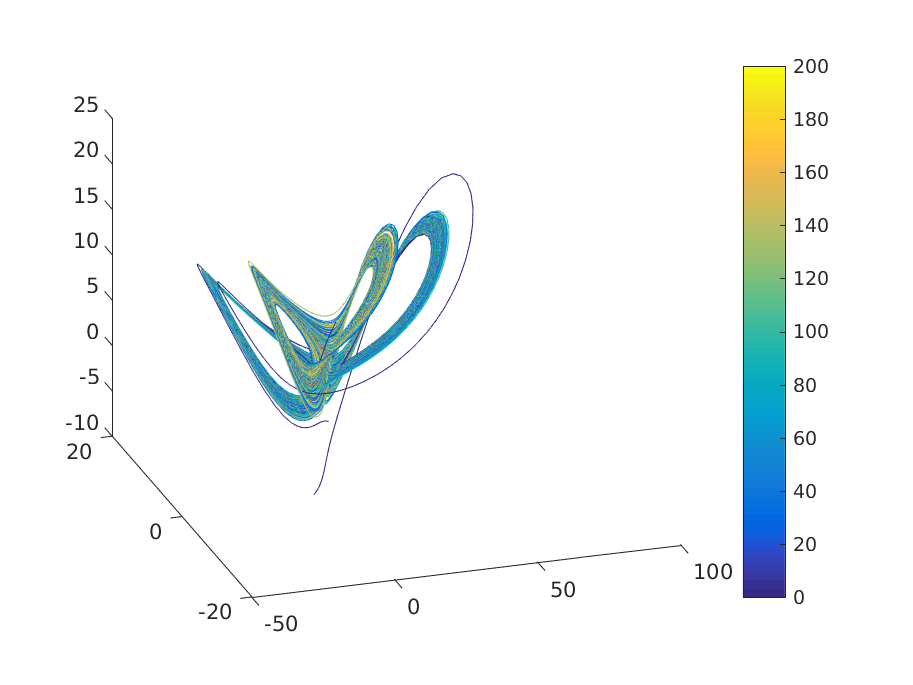
\includegraphics[width=\textwidth]{pictures/primera_simulacion}
		\caption{Resultado para primer caso de condiciones ininciales}
		\label{fig:simulacion1}
	\end{subfigure}
	\begin{subfigure}[b]{0.36\textwidth}
		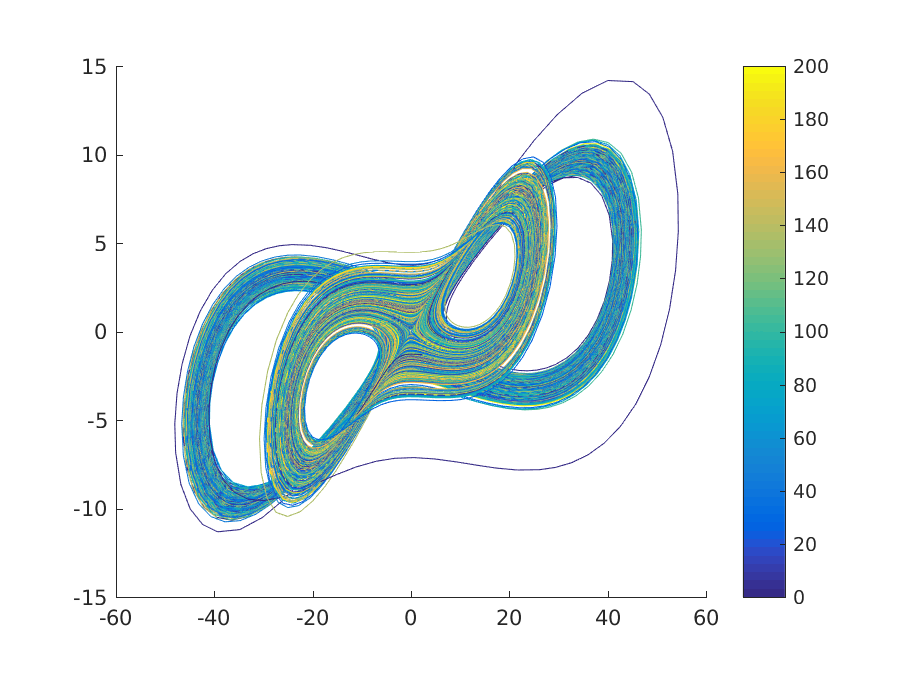
\includegraphics[width=\textwidth]{pictures/primera_simulacion_xy}
		\caption{Vista XY de la primera simulación}
		\label{fig:simulacion1xy}
	\end{subfigure}
        \vfill
        \begin{subfigure}[b]{0.36\textwidth}
		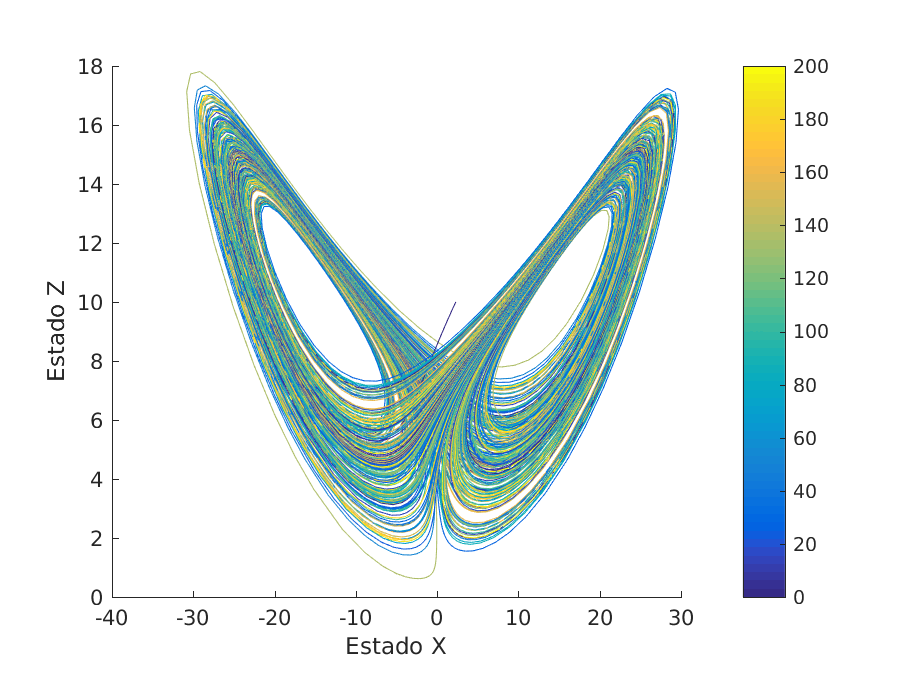
\includegraphics[width=\textwidth]{pictures/primera_simulacion_xz}
		\caption{Vista XZ de la primera simulación}
		\label{fig:simulacion1xz}
	\end{subfigure}

        \begin{subfigure}[b]{0.36\textwidth}
		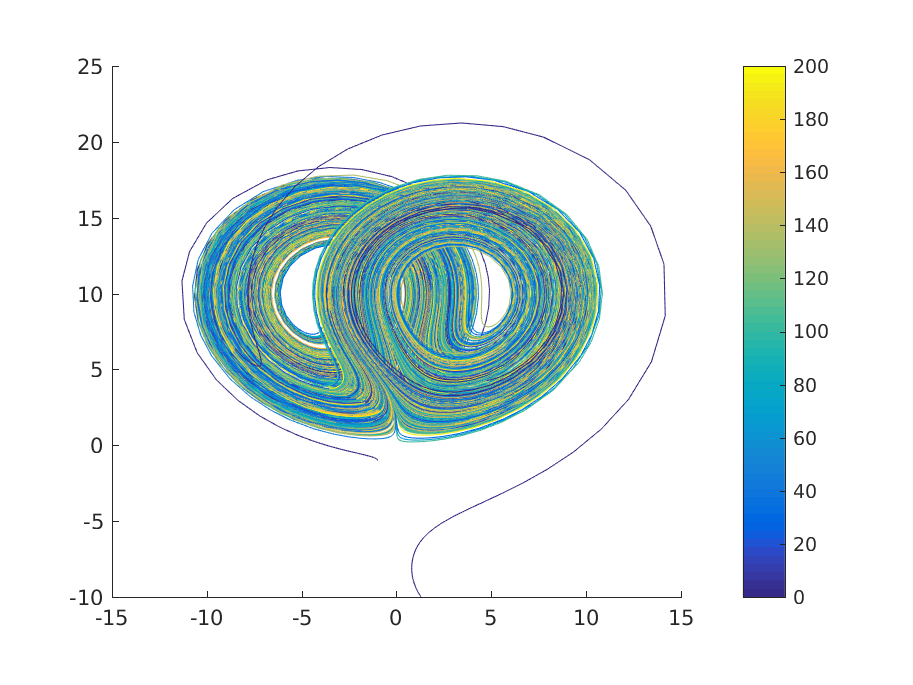
\includegraphics[width=\textwidth]{pictures/primera_simulacion_yz}
		\caption{Vista YZ de la primera simulación}
		\label{fig:simulacion1yz}
	\end{subfigure}
	\caption{Primera simulación gráfica de los estados. En los ejes se tienen los estados y el tiempo se denota con el cambio de color}
	\label{fig:simulacion1_total}
\end{figure}

%segunda simulacion ···········································································································································
\begin{figure}
	\centering
	\begin{subfigure}[b]{0.36\textwidth}
		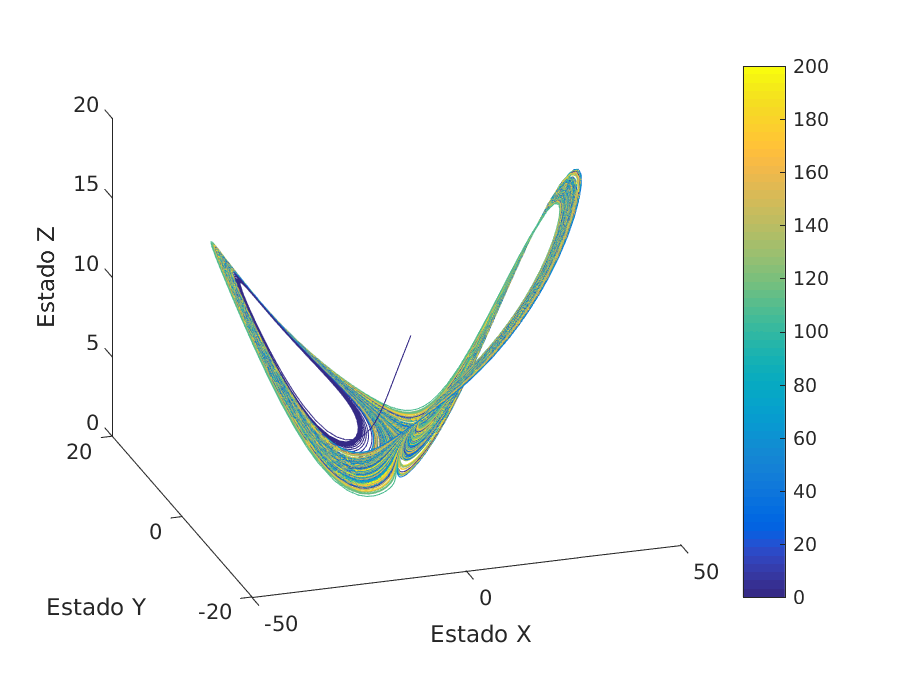
\includegraphics[width=\textwidth]{pictures/segunda_simulacion}
		\caption{Resultado para primer caso de condiciones ininciales}
		\label{fig:simulacion2}
	\end{subfigure}
	\begin{subfigure}[b]{0.36\textwidth}
		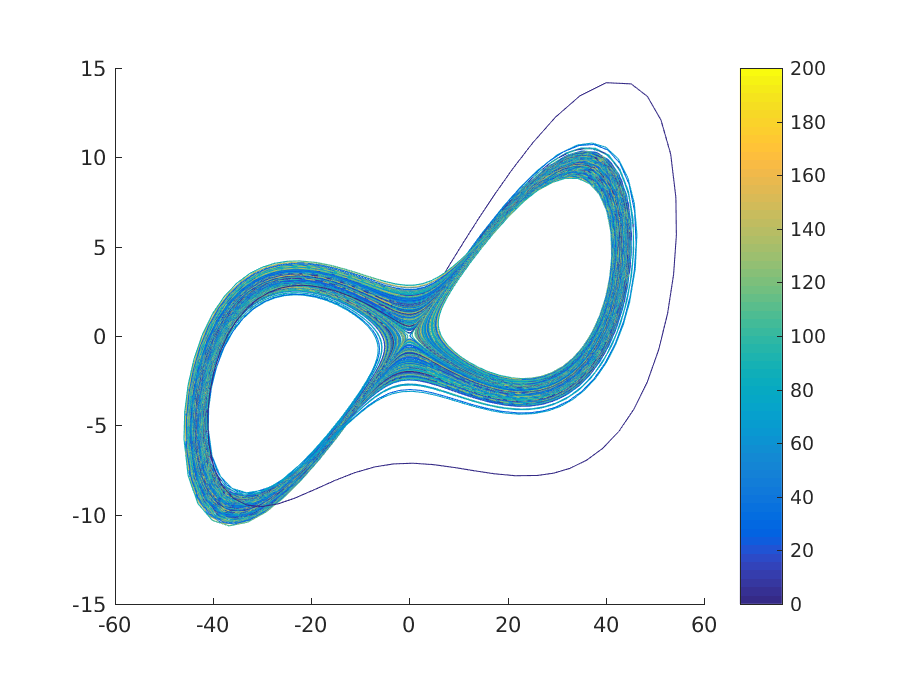
\includegraphics[width=\textwidth]{pictures/segunda_simulacion_xy}
		\caption{Vista XY de la segunda simulación}
		\label{fig:simulacion2xy}
	\end{subfigure}
        \vfill
        \begin{subfigure}[b]{0.36\textwidth}
		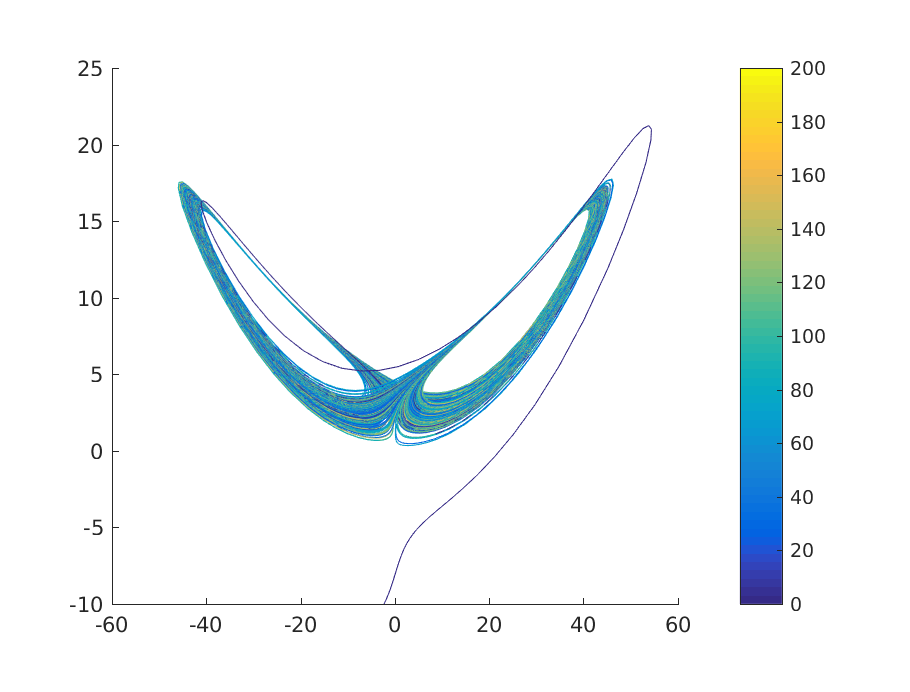
\includegraphics[width=\textwidth]{pictures/segunda_simulacion_xz}
		\caption{Vista XZ de la segunda simulación}
		\label{fig:simulacion2xz}
	\end{subfigure}

        \begin{subfigure}[b]{0.36\textwidth}
		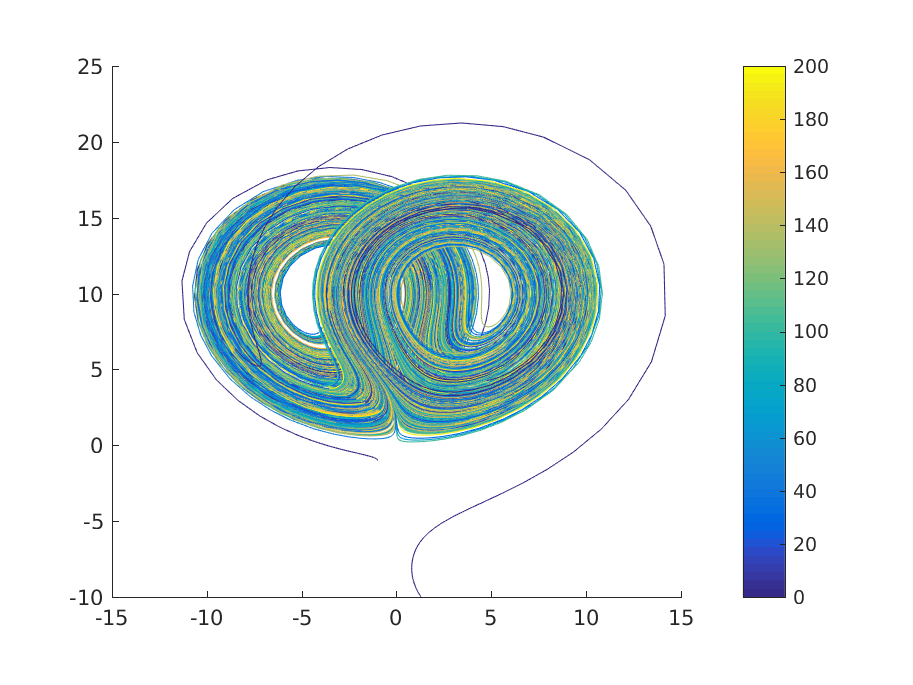
\includegraphics[width=\textwidth]{pictures/segunda_simulacion_yz}
		\caption{Vista YZ de la segunda simulación}
		\label{fig:simulacion2yz}
	\end{subfigure}
	\caption{Segunda simulación gráfica de los estados. En los ejes se tienen los estados y el tiempo se denota con el cambio de color}
	\label{fig:simulacion2_total}
\end{figure}

%Tercera simulacion ···········································································································································

\begin{figure}
	\centering
	\begin{subfigure}[b]{0.36\textwidth}
		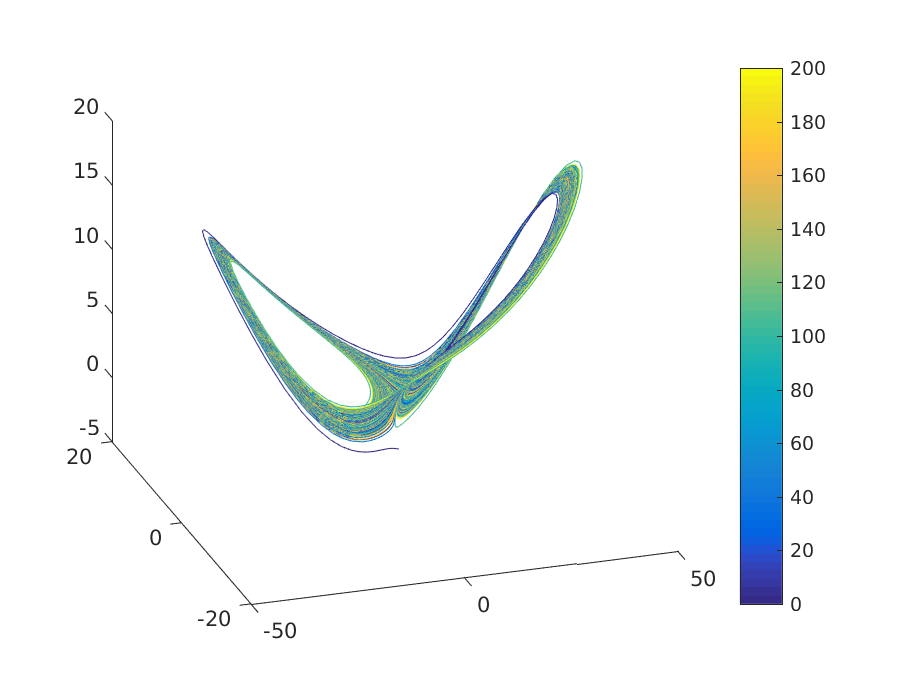
\includegraphics[width=\textwidth]{pictures/tercera_simulacion}
		\caption{Resultado para primer caso de condiciones ininciales}
		\label{fig:simulacion3}
	\end{subfigure}
	\begin{subfigure}[b]{0.36\textwidth}
		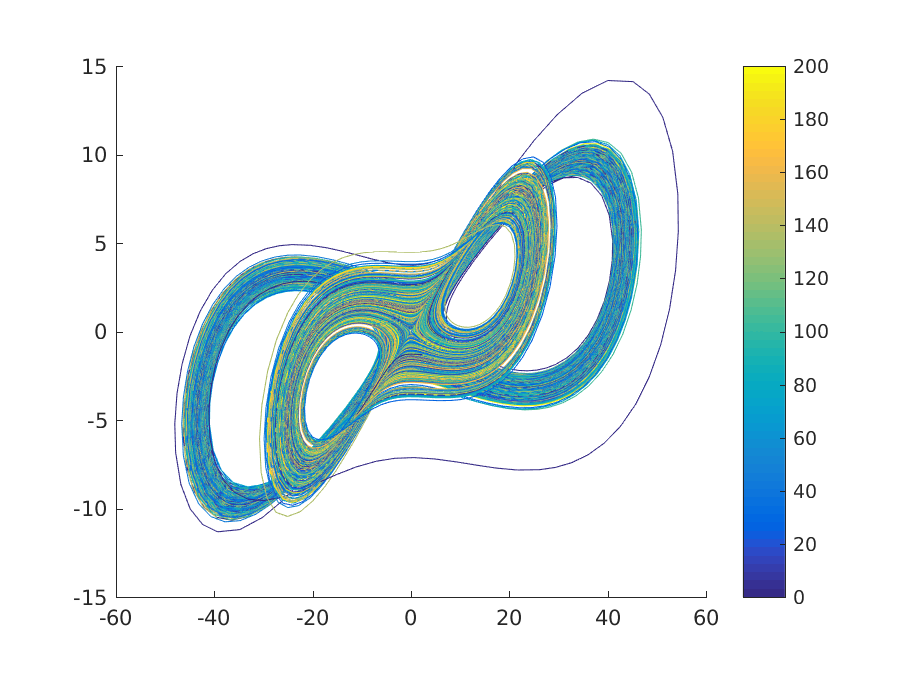
\includegraphics[width=\textwidth]{pictures/tercera_simulacion_xy}
		\caption{Vista XY de la tercera simulación}
		\label{fig:simulacion3xy}
	\end{subfigure}
        \vfill
        \begin{subfigure}[b]{0.36\textwidth}
		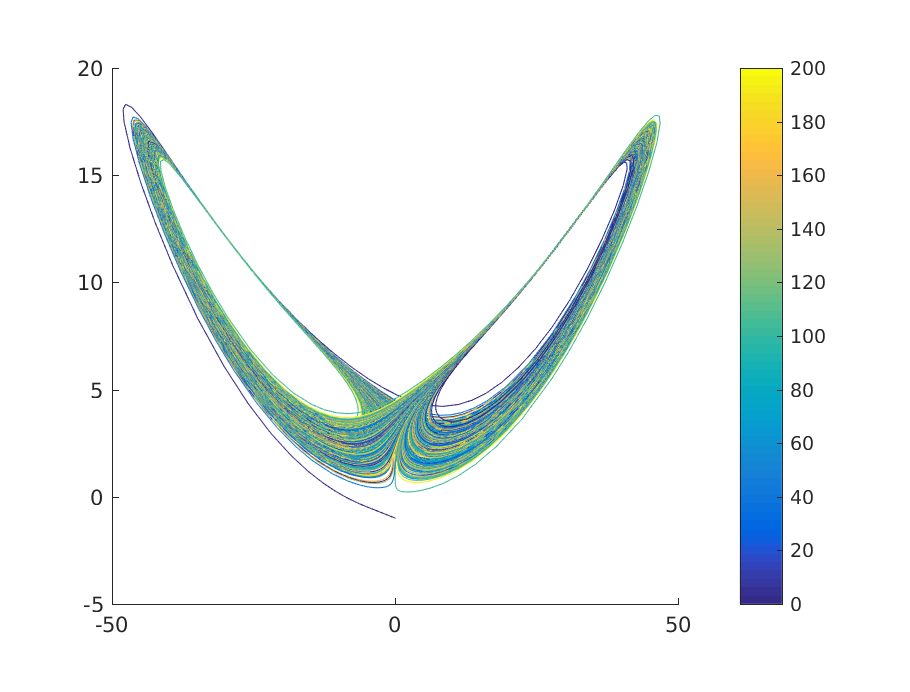
\includegraphics[width=\textwidth]{pictures/tercera_simulacion_xz}
		\caption{Vista XZ de la tercera simulación}
		\label{fig:simulacion3xz}
	\end{subfigure}

        \begin{subfigure}[b]{0.36\textwidth}
		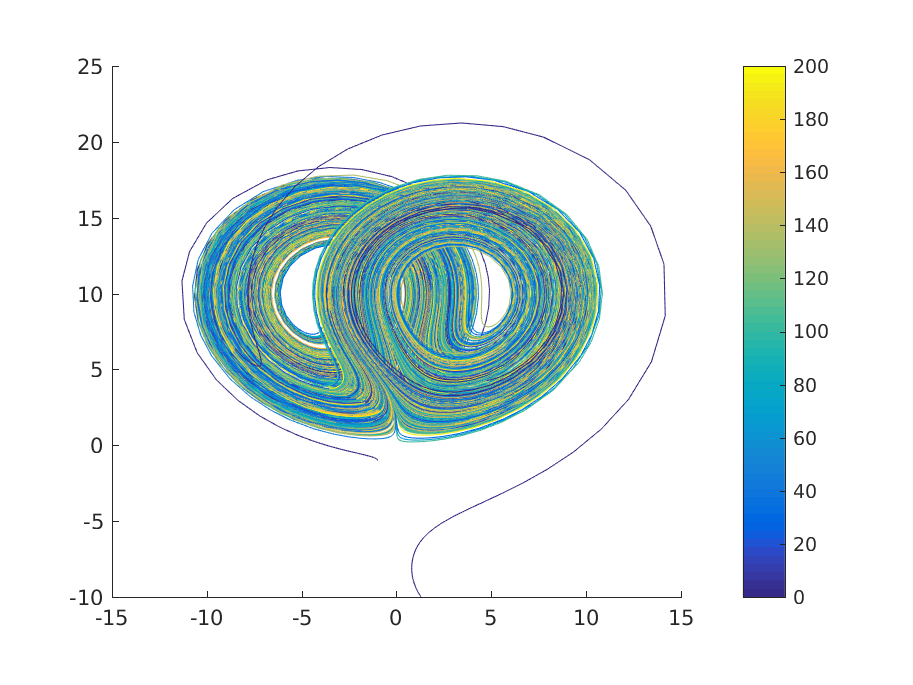
\includegraphics[width=\textwidth]{pictures/tercera_simulacion_yz}
		\caption{Vista YZ de la tercera simulación}
		\label{fig:simulacion3yz}
	\end{subfigure}
	\caption{Tercera simulación gráfica de los estados. En los ejes se tienen los estados y el tiempo se denota con el cambio de color}
	\label{fig:simulacion3_total}
\end{figure}

%Comparacion de los estados de las distintas simulaciones respecto al tiempo.···················································································

\begin{figure}
	\centering
<<<<<<< HEAD
	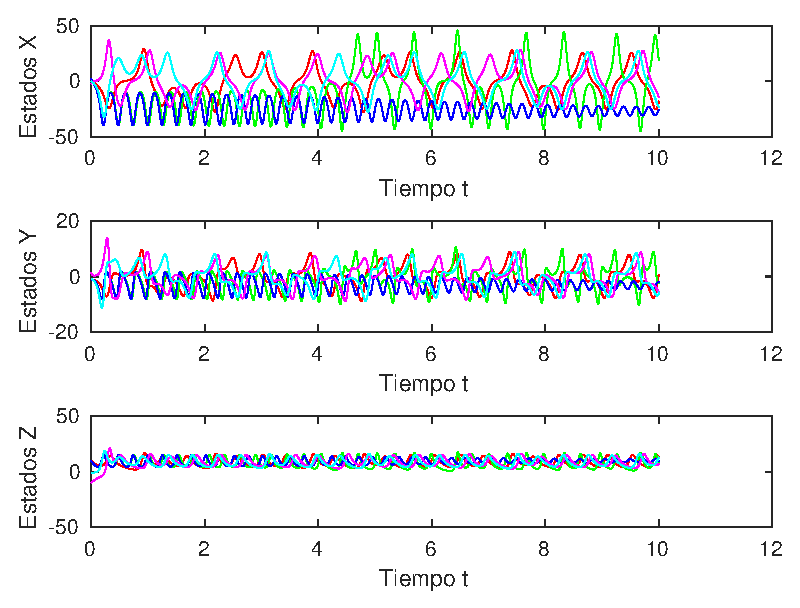
\includegraphics[width=\textwidth]{pictures/comparacion}
	\caption{Comparación de los estados de las distintas simulaciones respecto al tiempo}
=======
	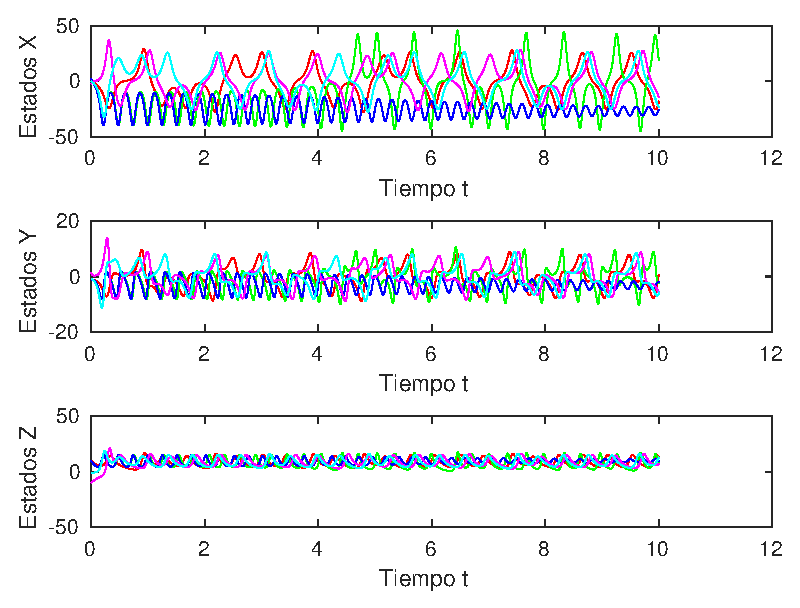
\includegraphics[width=0.8\textwidth]{pictures/comparacion}
	\caption{Comparación de los estados de las distintas simulaciones respecto al tiempo. Se presentan en rojo, verde, azul, magenta, y cían respectivamente cada simulación.}
>>>>>>> fdddc507e876d60fbe1cb246d378bef78c689287
	\label{fig:comparacion}
\end{figure}


<<<<<<< HEAD
=======
\begin{figure}
	\centering
	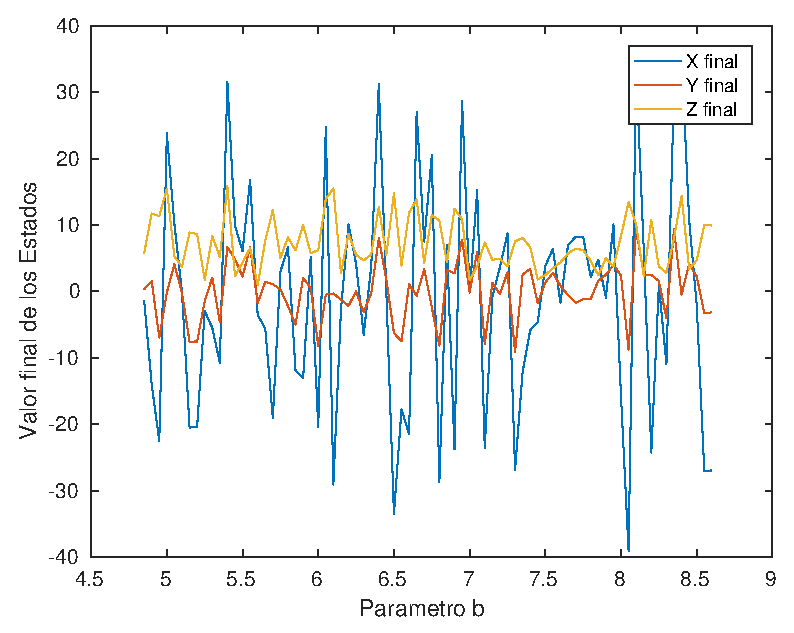
\includegraphics[width=0.8\textwidth]{pictures/sensibilidad}
	\caption{Valor final de cada estado, dependiendo del valor de b}
	\label{fig:sensibilidad}
\end{figure}
>>>>>>> fdddc507e876d60fbe1cb246d378bef78c689287

\subsubsection{Código de ejercicio 1}



\section{Ejercicio 2}

De las ecuaciones de corriente en el diodo \eqref{eq:Id_diodo} y voltaje en el diodo  \eqref{eq:Vd_diodo}

\begin{equation}
\label{eq:Id_diodo}
I_d=I_s(e^{\frac{V_d}{nV_t}}-1)
\end{equation}



\begin{equation}\label{eq:Vd_diodo}
V_d= V_{in}-V_o
label{eq:Id_diodo}
\end{equation}

Se obtiene el siguiente desarrollo mediante ley de corrientes de kirkchoff 

\begin{equation}
SCV_o + \frac{V_o}{R} = I_d
\end{equation}

\begin{equation}
C \frac{dV_o}{dt} + \frac{V_o}{R} = I_s\left(e^{\frac{V_d}{nV_t}}-1\right)
\end{equation}

\begin{equation}
C \frac{dV_o}{dt} + \frac{V_o}{R} = I_s\left(e^{\frac{V_{in}-V_{o}}{nV_t}}-1\right)
\end{equation}

A partir de las ecuaciones anteriores se obtuvo el diagrama de bloques presente en la figura \ref{fig:diag_bloques_2}


\begin{figure}[ht!]
  \centering
  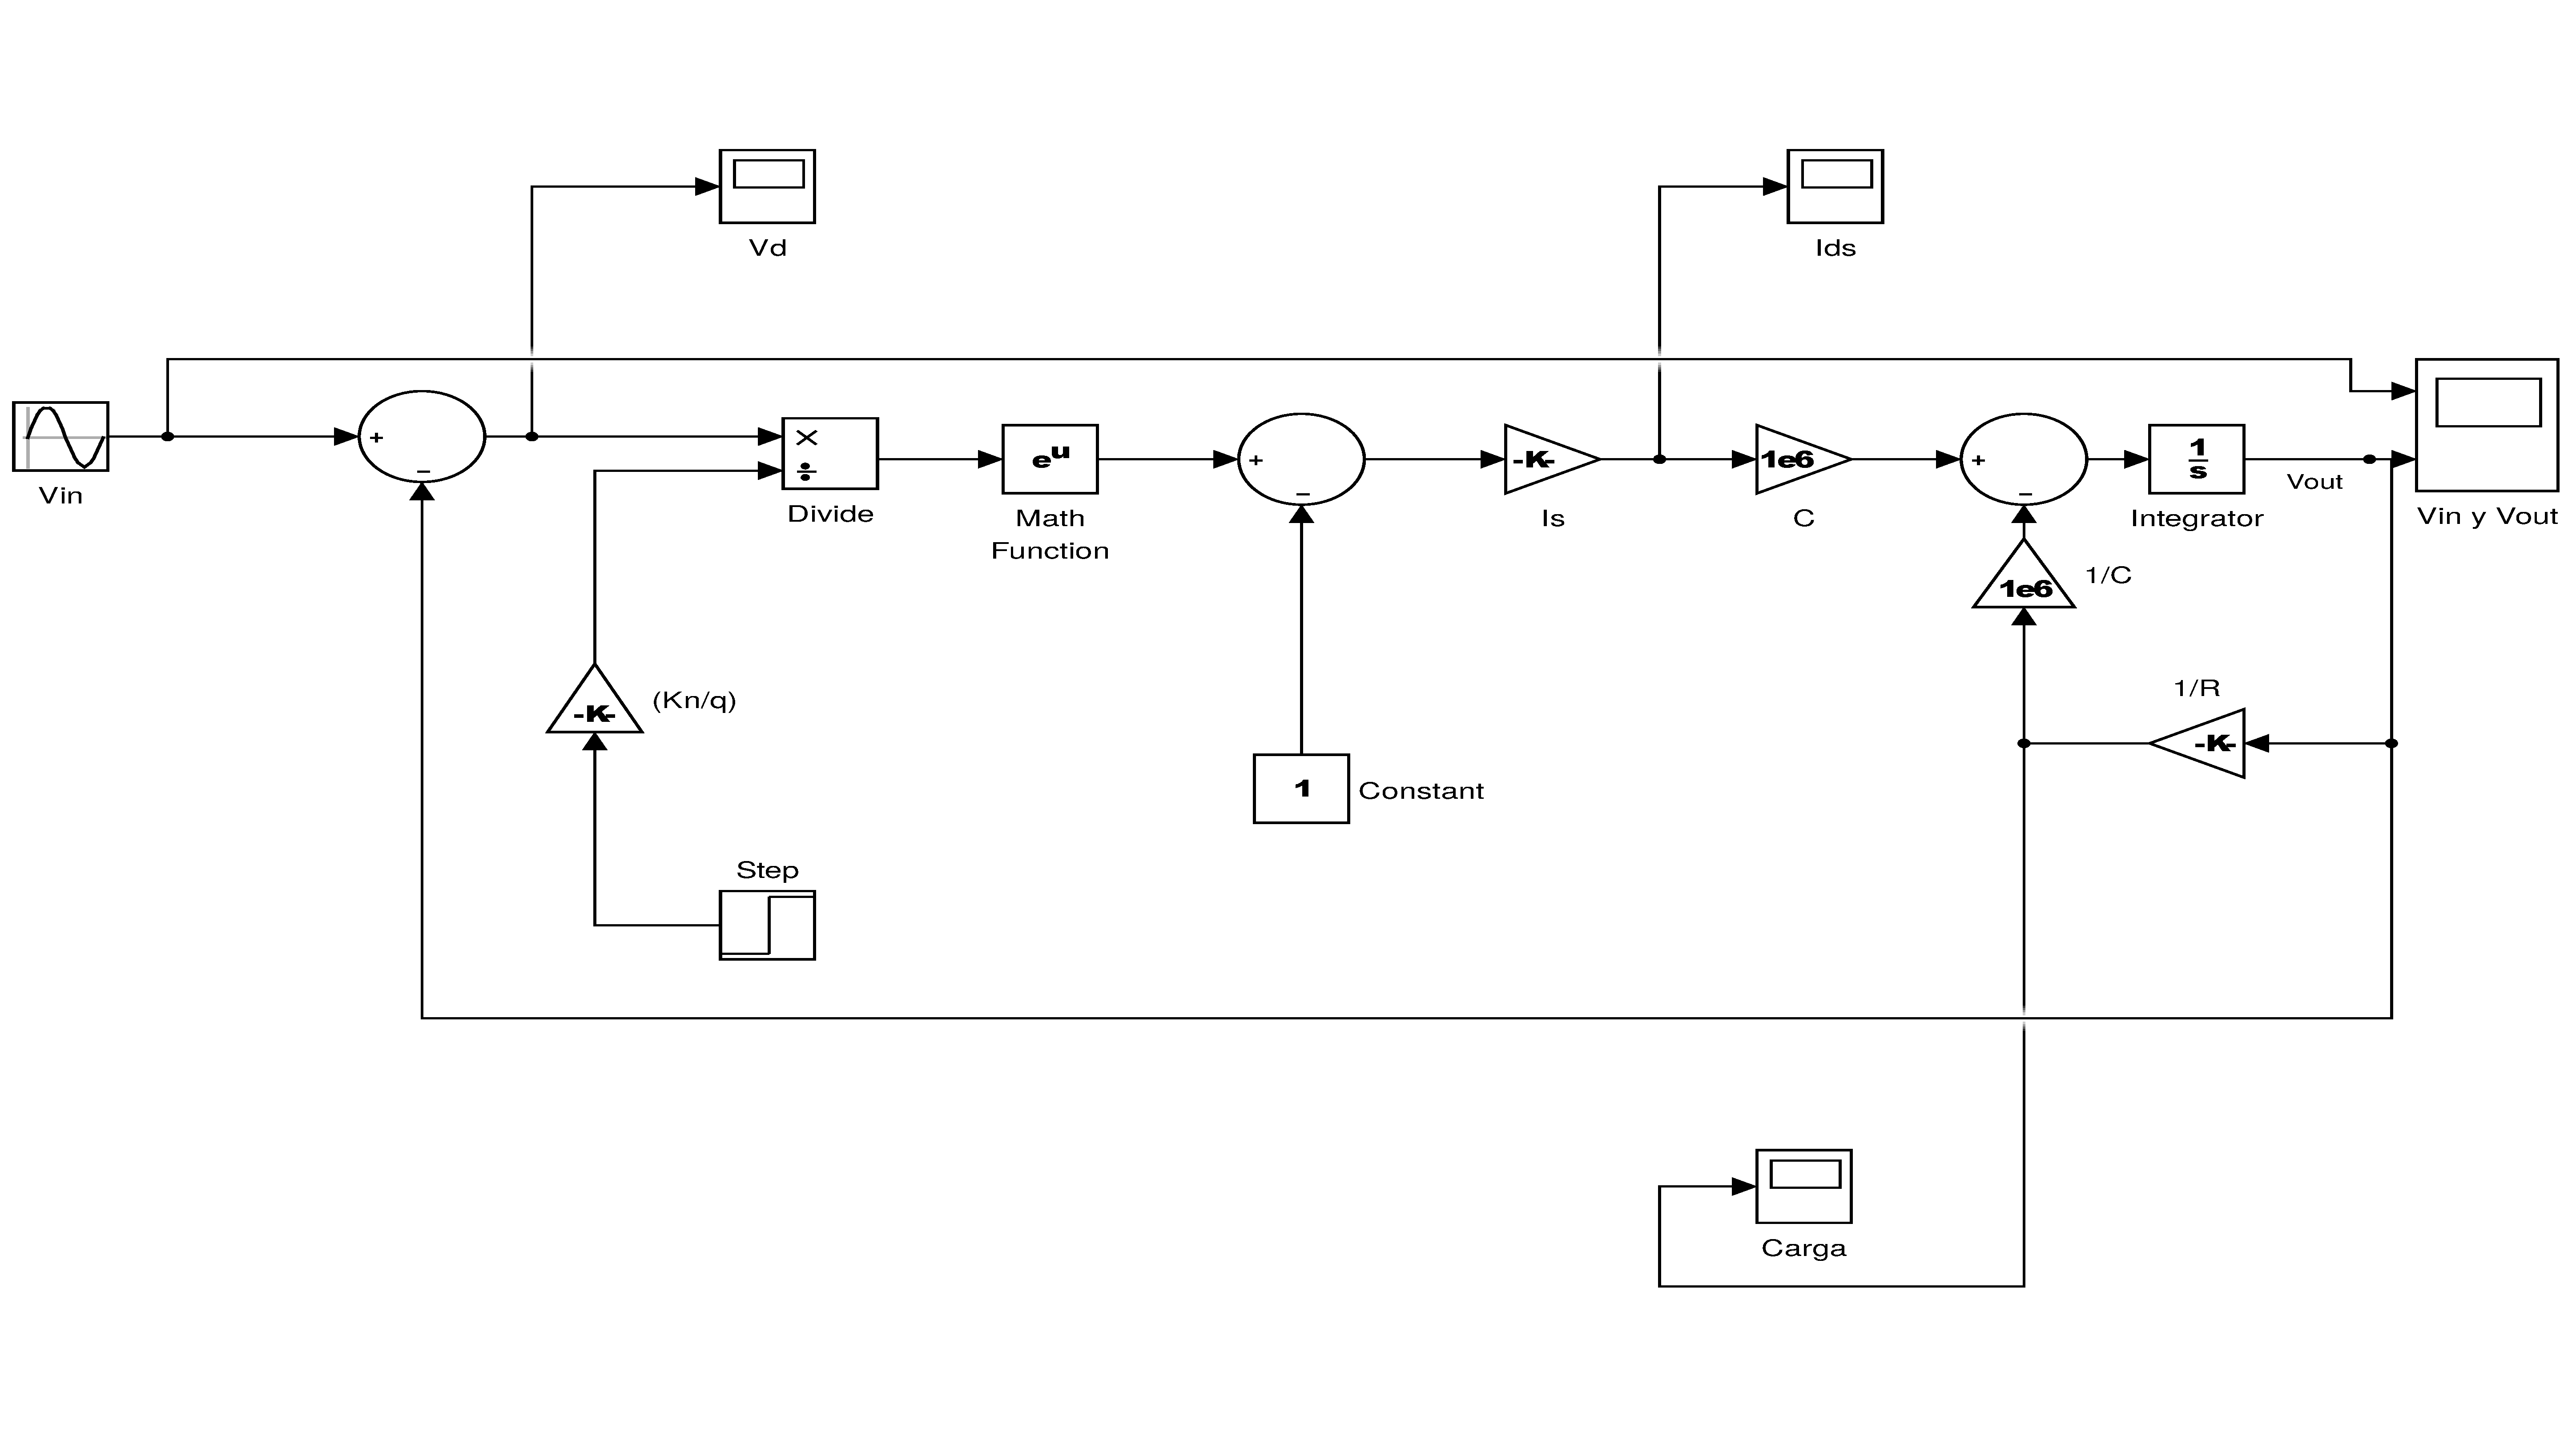
\includegraphics[width=0.8\linewidth]{pictures/Ejercicio2_Diagrama_Bloques.eps}
  \caption{Diagrama de bloques en Simulink}
  \label{fig:diag_bloques_2}
\end{figure}

A continuación simulamos las condiciones dadas para cada punto (a, b y c) haciendo leves variaciones en la estructura y parametros de los bloques.

\subsection{Parte A}
A continuación se presentan las gráficas obtenidas en la simulación para este punto. 

\begin{figure}[ht!]
  \centering
  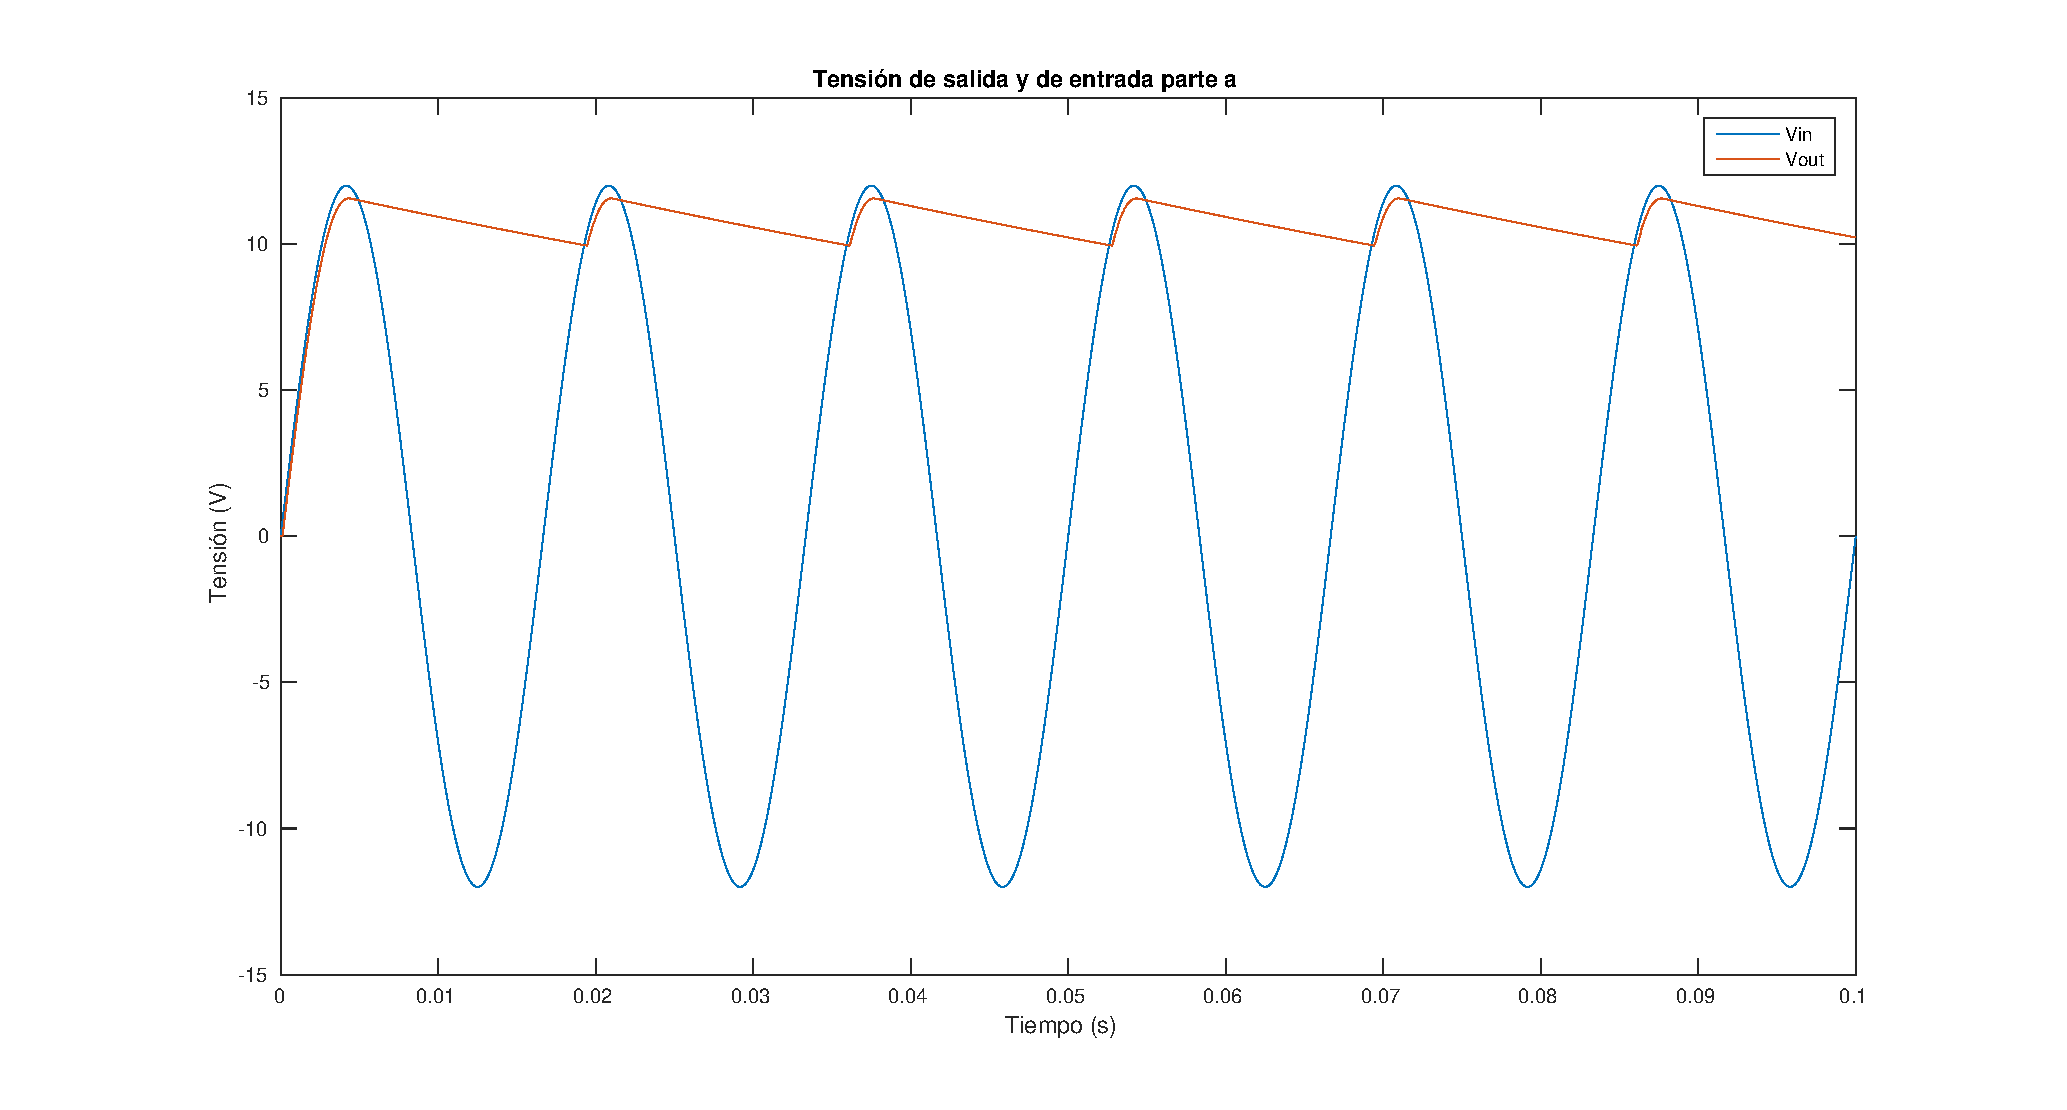
\includegraphics[width=0.8\linewidth]{pictures/Ejercicio2_a_Vin_Vout.eps}
  \caption{Tension }
  \label{fig:2_a_Vin_Vout}
\end{figure}

En la figura \ref{fig:2_a_Vin_Vout} se puede observar que la gráfica cumple de acuerdo a lo descrito en la teoría, ya que la onda de salida solo posee fase positiva, esto se debe al diodo que se colocó, pues únicamente deja pasar la fase positiva de la onda, si lo relacionamos con el diagrama de bloques obtenido, al ser negativo la parte exponencial de la ecuación obtenida  se hace tan pequeña que podemos considerarla nula por lo que a la entrada de nuestro sumador solo está el "-1" y al multiplicarlo por la corriente de saturación inversa del diodo ($I_s$) tenemos un valor tan pequeño que es considerable cero. Además de esto el capacitor es el encargado de mantener un voltaje de rizado en la onda y que no caiga por completo, pues representa una ganancia considerable a la entrada del bloque sumador de Vout que viene de la corriente, aunque también representa una ganancia para la retroalimentación negativa, sin embargo este ultimo efecto es atenuado por la resistencia de carga.

\begin{figure}[ht!]
  \centering
  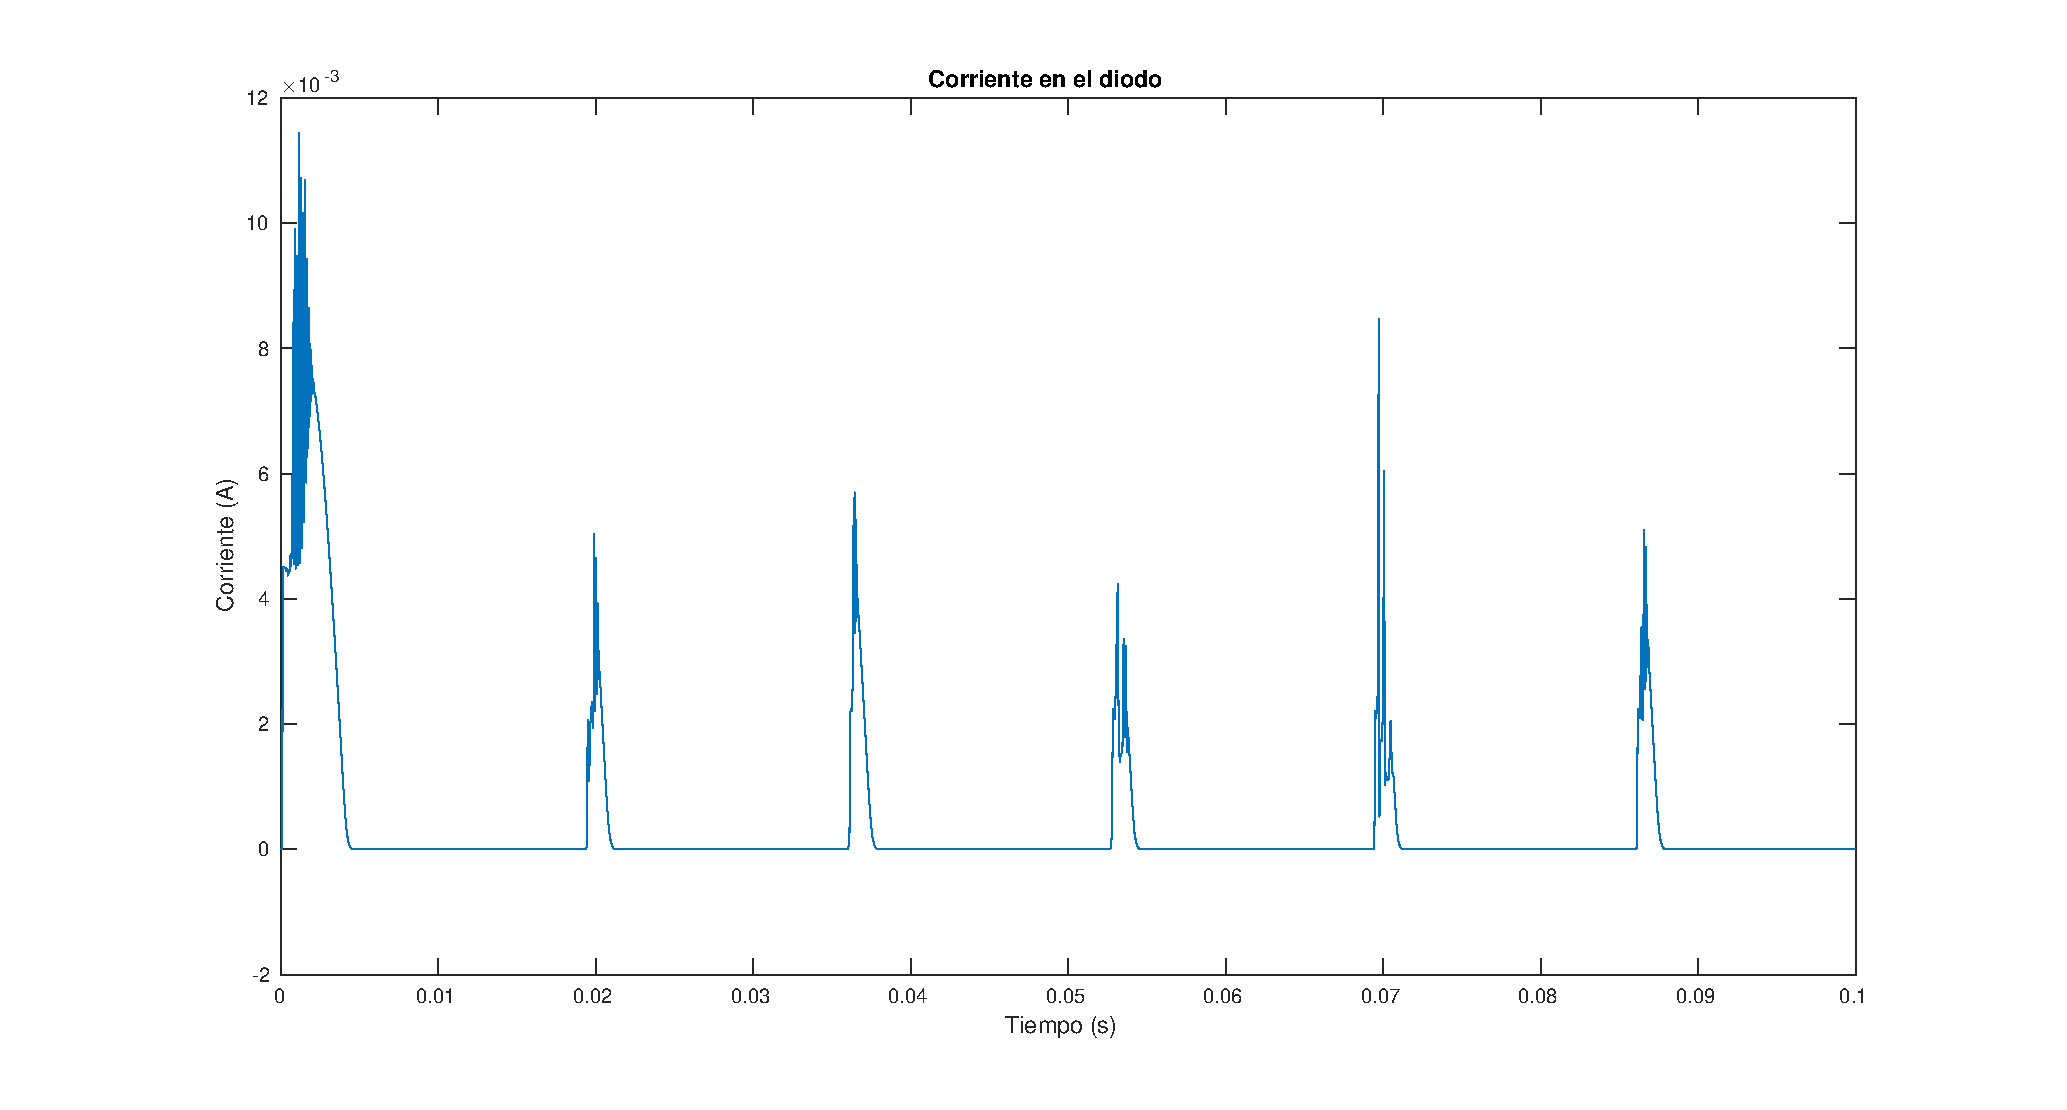
\includegraphics[width=0.8\linewidth]{pictures/Ejercicio2_a_corriente_diodo.eps}
  \caption{Corriente en el diodo}
  \label{fig:2_a_Id}
\end{figure}

Ahora se muestra en la figura \ref{fig:2_a_Id} la corriente que pasa por el diodo, como era de esperarse los picos de corriente máxima que se alcanzan coinciden o al menos están bastante cerca de la tensión máxima en la entrada por lo ya explicado anteriormente. Por otro lado, la corriente es cero en la fase negativa de la onda como se esperaba. Podemos decir que la gráfica refleja la ecuación de la corriente, ya que crece de manera exponencial y por eso es que vemos un pico.

\begin{figure}[ht!]
  \centering
  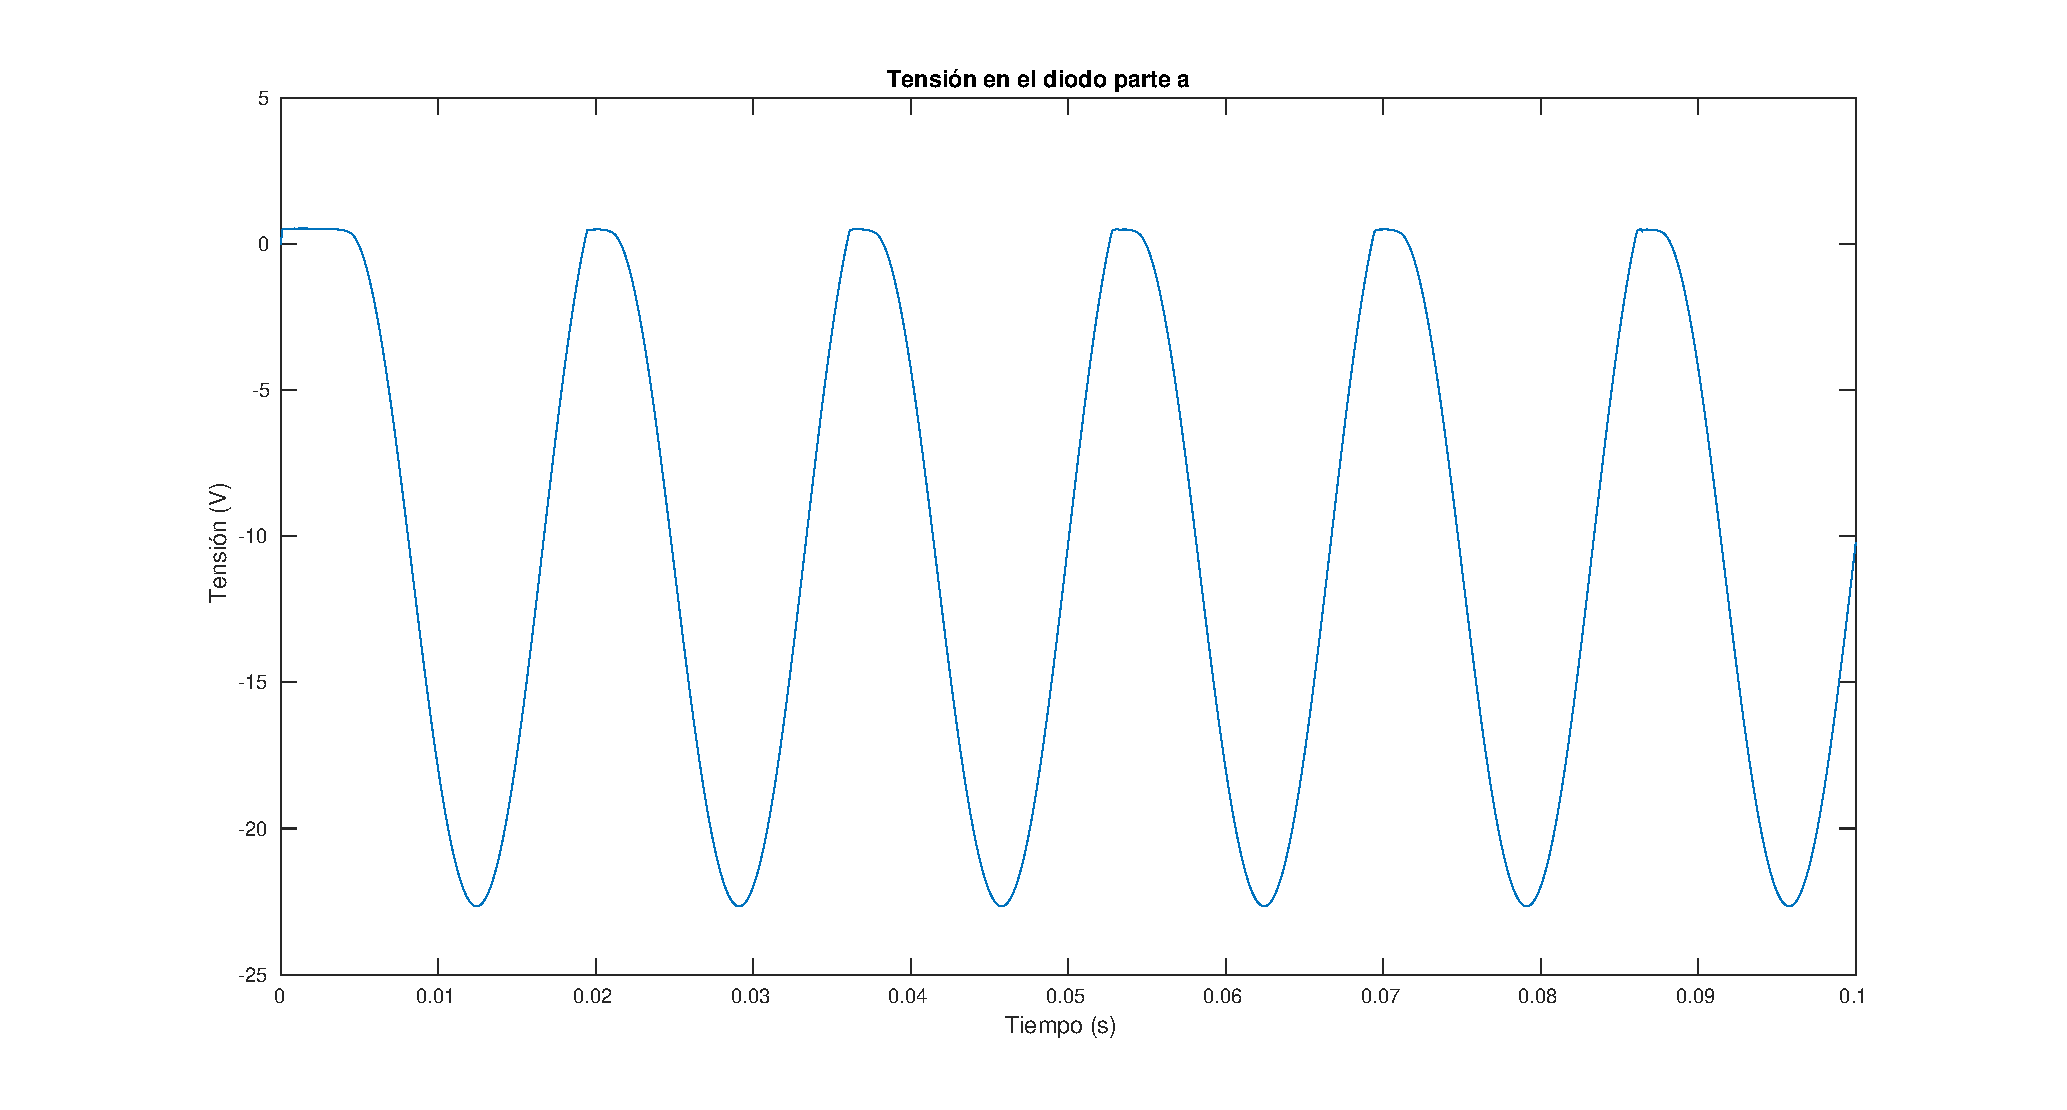
\includegraphics[width=0.8\linewidth]{pictures/Ejercicio2_a_Vd.eps}
  \caption{Voltaje en el diodo}
  \label{fig:2_a_Vd}
\end{figure}

Al ser $V_d = V_{in}-V_{out}$ corresponderá a casi el doble pero de manera negativa, ya que de la figura \ref{fig:2_a_Vin_Vout} se obtuvo que el voltaje, cuando la fase es negativa, es suministrado por el capacitor. Así que como $V_{in} < 0$ y $V_{out} > 0$ se obtuvo la gráfica de la figura \ref{fig:2_a_Vd}

\begin{figure}[ht!]
  \centering
  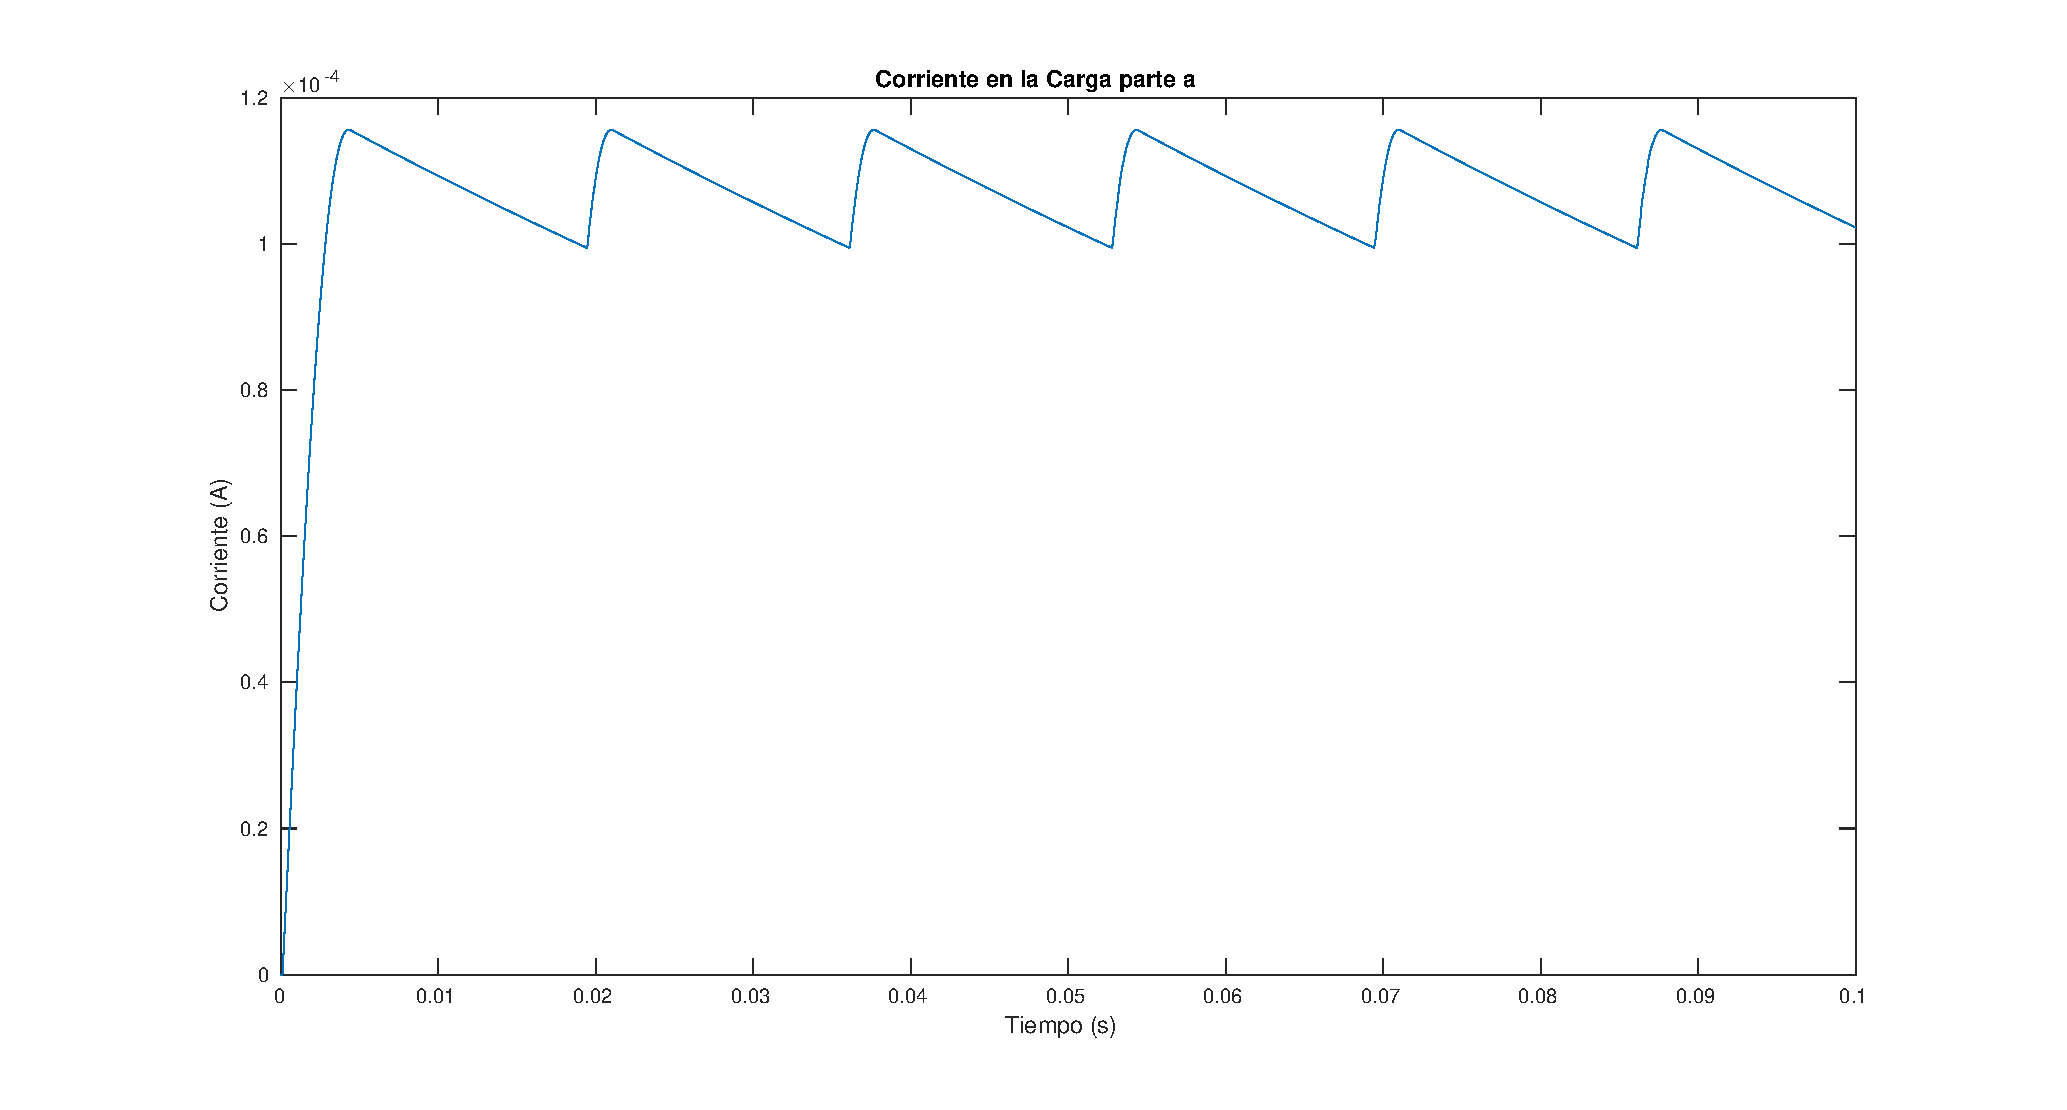
\includegraphics[width=0.8\linewidth]{pictures/Ejercicio2_a_carga.eps}
  \caption{Diagrama de bloques en Simulink}
  \label{fig:2_a_carga}
\end{figure}
Para la carga ,por ley de ohm, si el voltaje de salida varía la corriente de carga lo hace de igual manera, obteniendo así la misma forma que la gráfica de salida del voltaje que en la figura \ref{fig:2_a_Vin_Vout}. 

\subsection{Parte B}

A continuación se presentan las gráficas obtenidas en la simulación para este punto.

\begin{figure}[ht!]
  \centering
  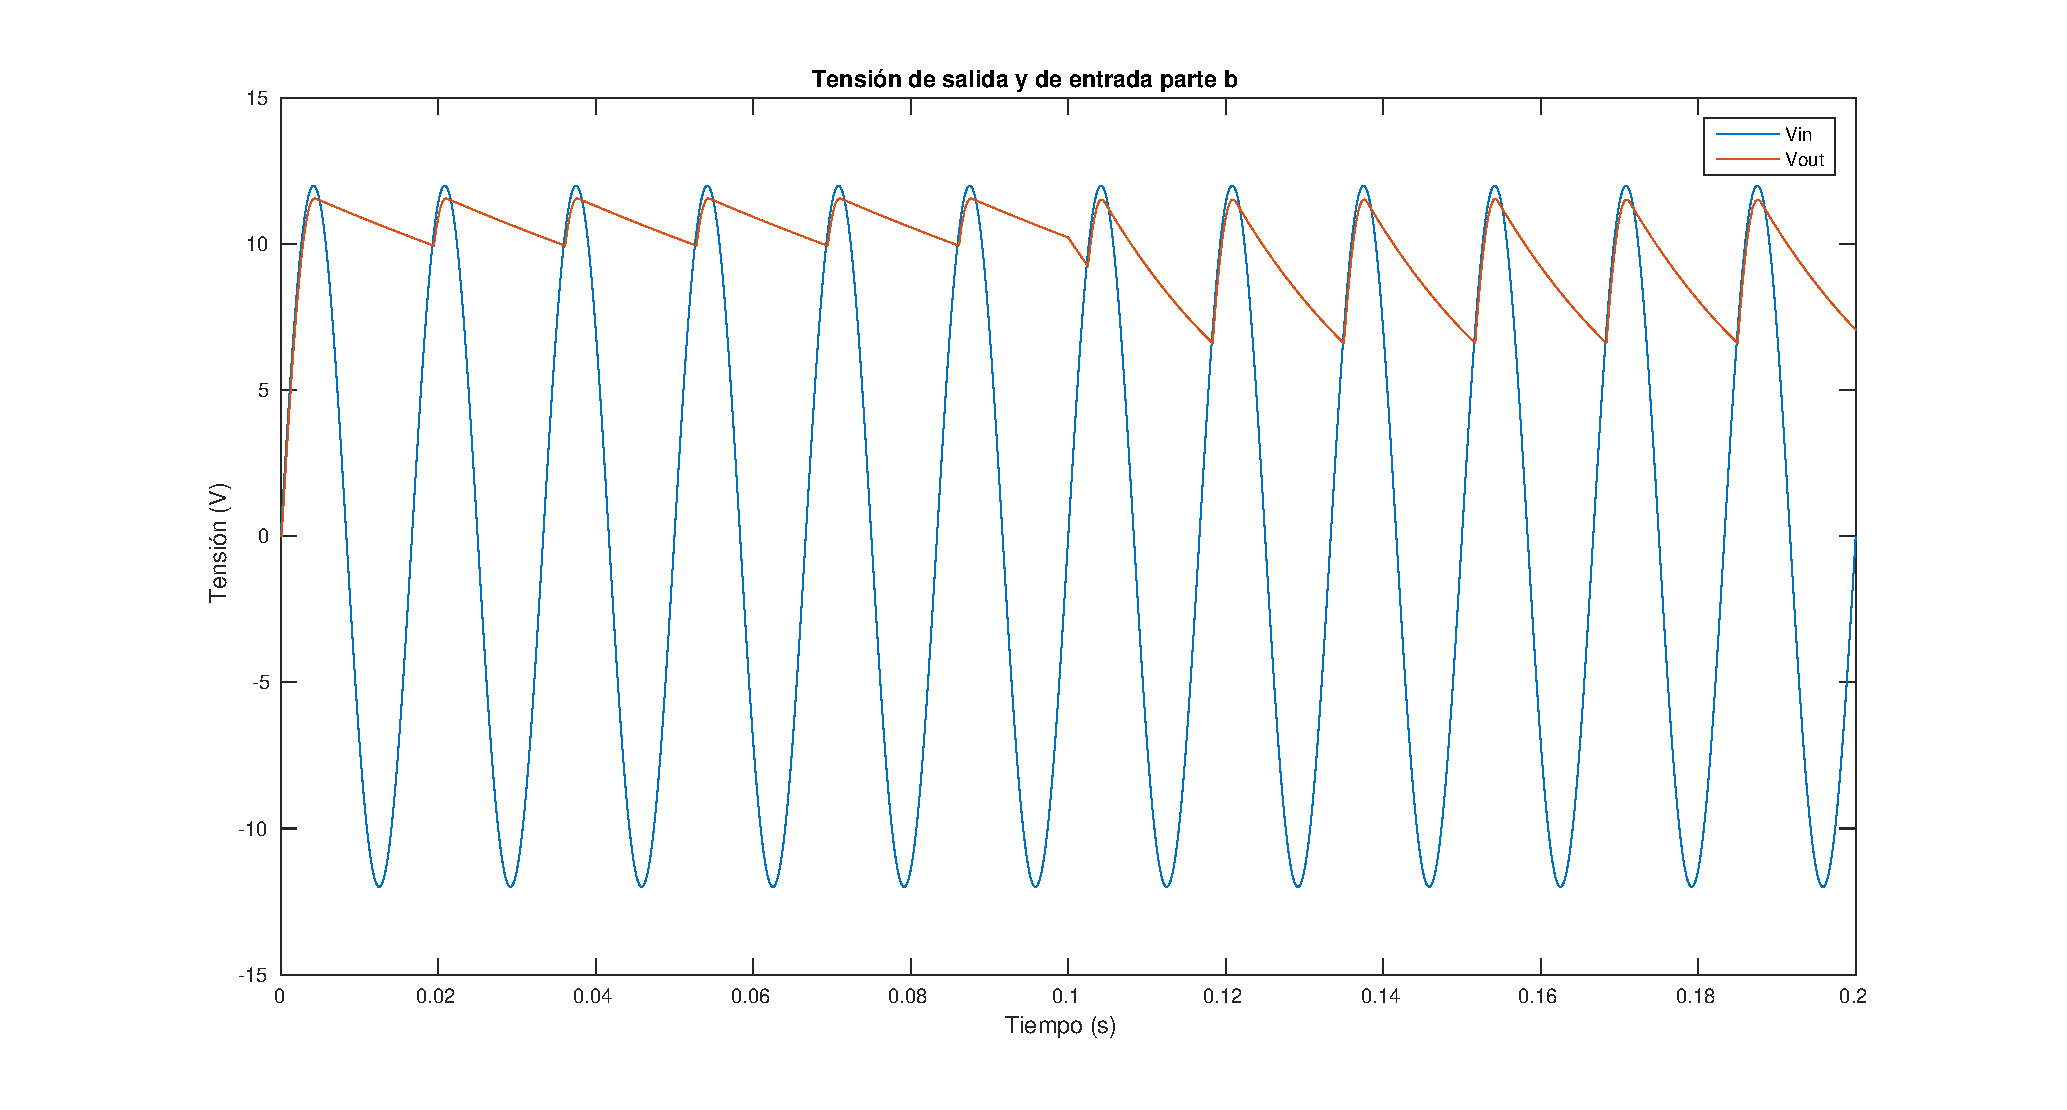
\includegraphics[width=0.8\linewidth]{pictures/Ejercicio2_b_Vin_Vout.eps}
  \caption{Tension de salida y entrada }
  \label{fig:2_b_Vin_Vout}
\end{figure}

Al variar la carga de manera instantánea, esto refleja un aumento en la retroalimentación negativa de $V_{out}$ ya que la resistencia atenuaba la ganancia del capacitor en la retroalimentación negativa, por eso es que $V_{out}$ decae un poco más, es decir el rizado aumentó. Viendolo desde el punto de vista más físico lo que está ocurriendo es que al disminuir la resistencia el capacitor entrega mayor corriente por lo que se descarga más rapido. Esto corresponde con la gráfica de la figura \ref{fig:2_b_Vin_Vout}

\begin{figure}[ht!]
  \centering
  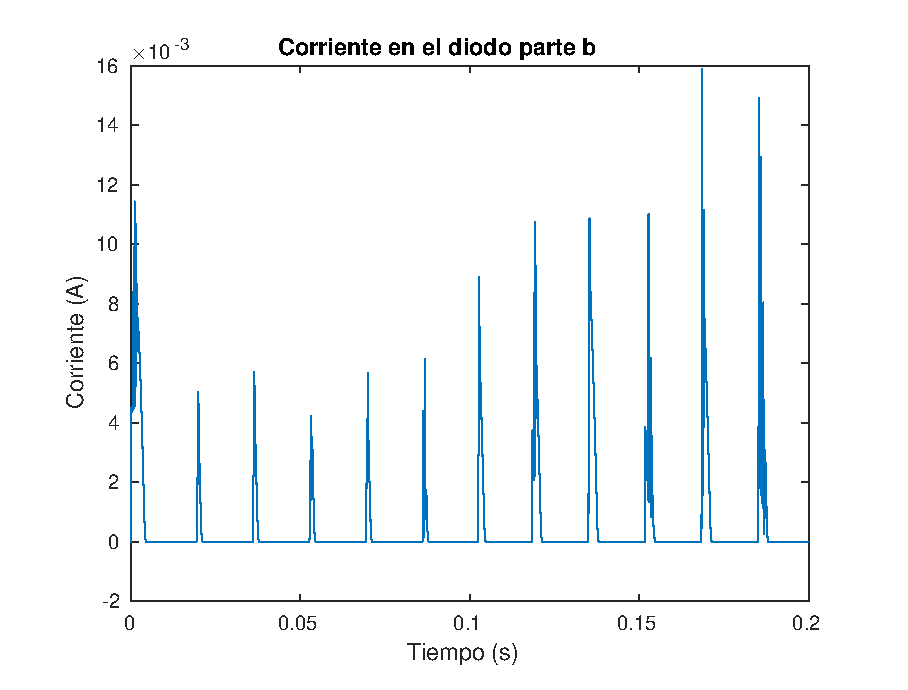
\includegraphics[width=0.8\linewidth]{pictures/Ejercicio2_b_corriente_diodo.eps}
  \caption{Corriente en el diodo}
  \label{fig:2_b_Id}
\end{figure}

En este caso, como disminuye la resistencia aumenta la corriente en el diodo, ya que al disminuir $V_{out}$ el capacitor se descarga más rapido, la corriente aumenta según la ecuación \eqref{eq:Id_diodo} de esta forma se muestra la gráfica en la figura \ref{fig:2_b_Id}

\begin{figure}[ht!]
  \centering
  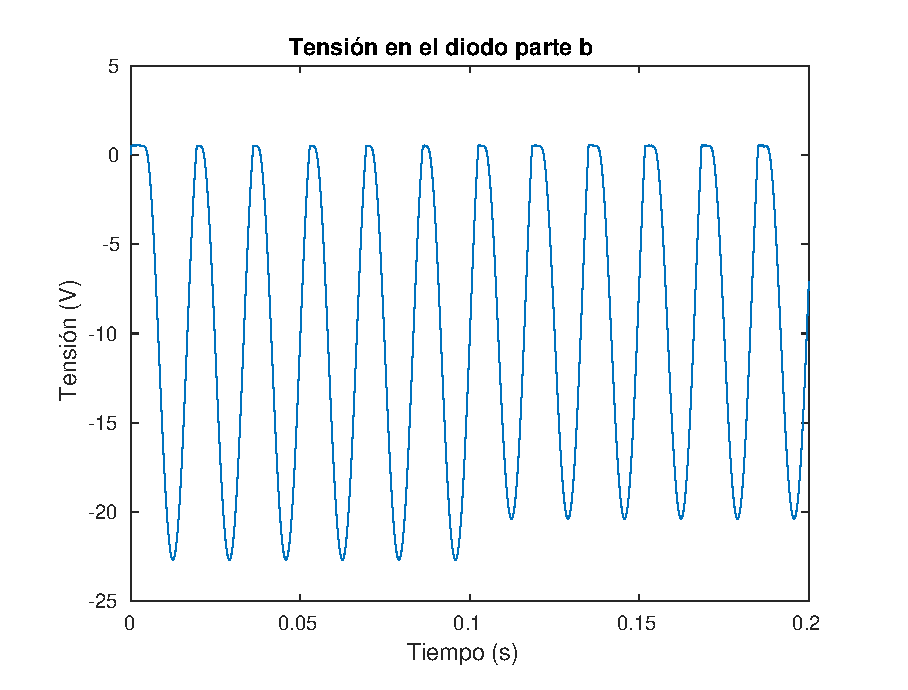
\includegraphics[width=0.8\linewidth]{pictures/Ejercicio2_b_Vd.eps}
  \caption{Voltaje en el diodo}
  \label{fig:2_b_Vd}
\end{figure}

En este como el voltaje de salida disminuye, el voltaje en el diodo también de acuerdo a la ecuación \eqref{eq:Vd_diodo} pues al decaer más el voltaje de salida en la fase negativa de la entrada hace que se reduzca su amplitud, sin embargo en la fase positiva permanece igual.

\begin{figure}[ht!]
  \centering
  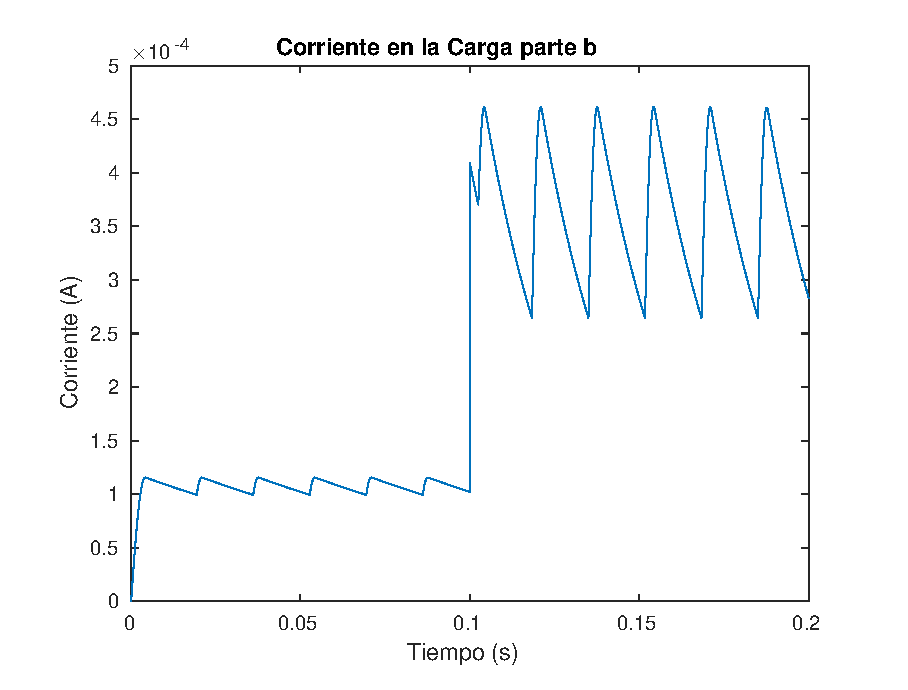
\includegraphics[width=0.8\linewidth]{pictures/Ejercicio2_b_carga.eps}
  \caption{Corriente de carga}
  \label{fig:2_b_carga}
\end{figure}

Como la carga disminuyó es razonable pensar que el capacitor está obligado a entregar más corriente para lograr mantener el voltaje máximo, por lo que a esto se debe el aumento de corriente que caracteriza esta curva, y siempre mantiene la forma de $V_{out}$, obteniendo así la gráfica de la figura \ref{fig:2_b_carga}


\subsection{Parte C}

Se presenta ahora las gráficas para esta sección, en este caso la temperatura en el diodo variaba de manera lineal.

\begin{figure}[ht!]
  \centering
  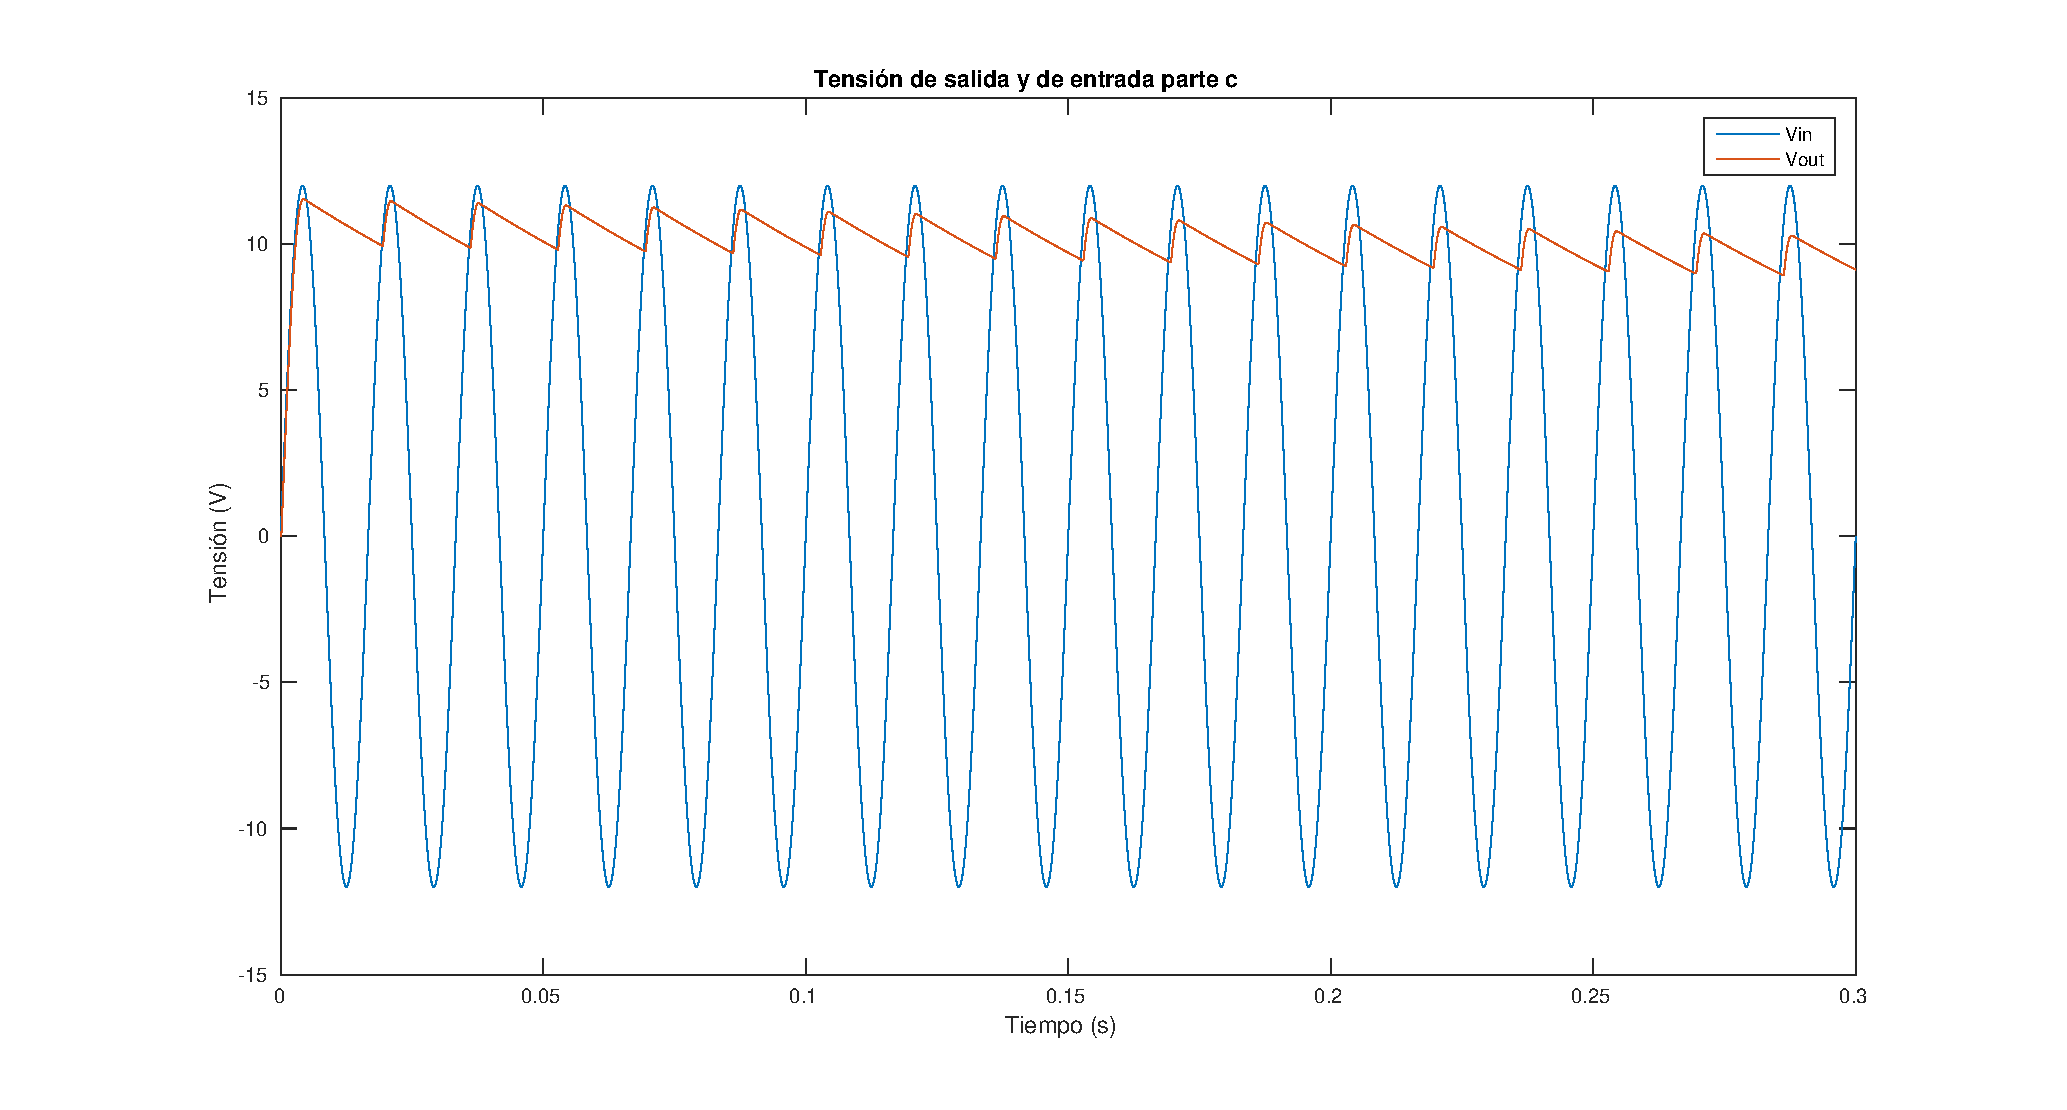
\includegraphics[width=0.8\linewidth]{pictures/Ejercicio2_c_Vin_Vout.eps}
  \caption{Tension de salida y entrada }
  \label{fig:2_c_Vin_Vout}
\end{figure}

Se observa en la gráfica el efecto de la temperatura en el diodo, a partir de la gráfica se puede decir que el efecto de la temperatura en el diodo no es tan determinante como el de las otras variables del cual depende el voltaje de salida. Esto debido a que debería llegar a un temperatura considerablemente alta (1200 k) para lograr obtener un efecto más apreciable.

\begin{figure}[ht!]
  \centering
  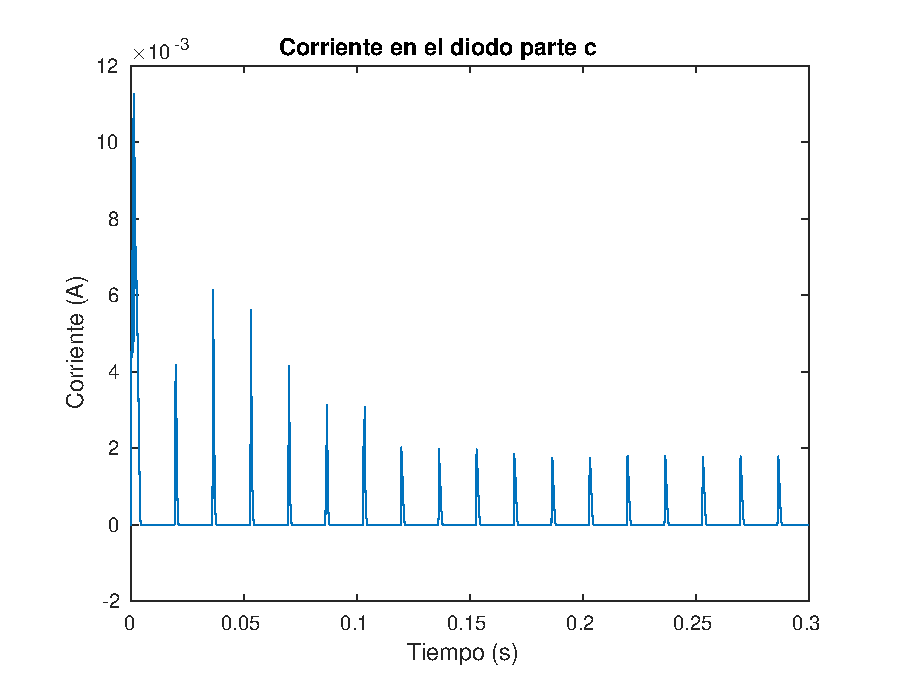
\includegraphics[width=0.8\linewidth]{pictures/Ejercicio2_c_corriente_diodo.eps}
  \caption{Corriente en el diodo}
  \label{fig:2_c_Id}
\end{figure}

Para el caso de la corriente en el diodo se tiene la gráfica de la figura \ref{fig:2_c_Id} donde se puede apreciar que existe un punto donde la temperatura deja de tener efecto sobre la corriente ya que el valor de esta parece estabilizarse. Aunque al inicio su efecto es bastante importante ya que el siguiente pico decayó bastante

\begin{figure}[ht!]
  \centering
  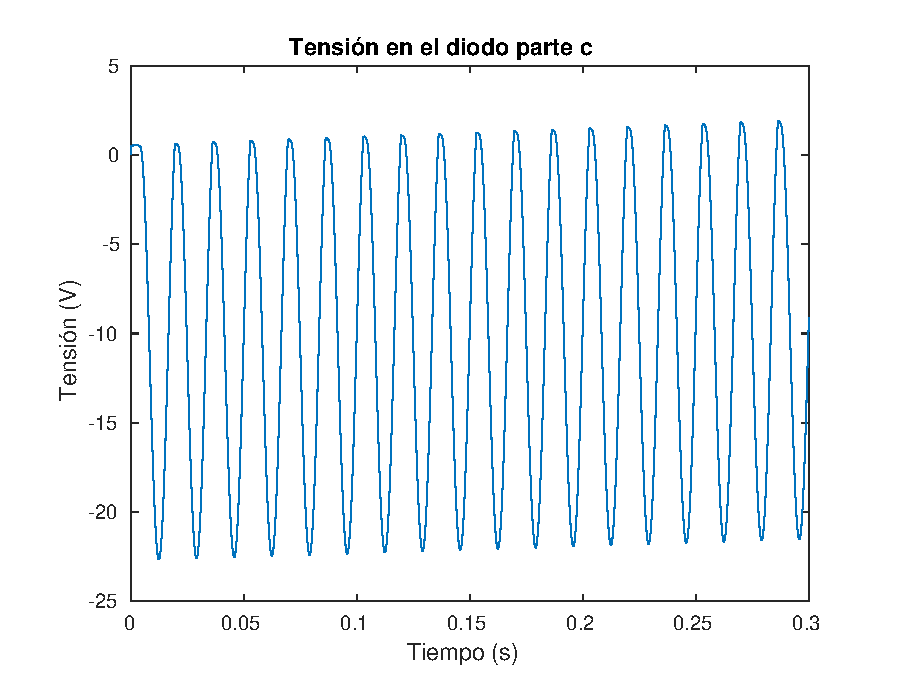
\includegraphics[width=0.8\linewidth]{pictures/Ejercicio2_c_Vd.eps}
  \caption{Voltaje en el diodo}
  \label{fig:2_c_Vd}
\end{figure}

Sobre la tensión del diodo tampoco parece tener un efecto muy significativo el cambio de temperatura sin embargo parece tener una leve disminución en la amplitud al final de la gráfica presente en la figura \ref{fig:2_c_Vd}

\begin{figure}[ht!]
  \centering
  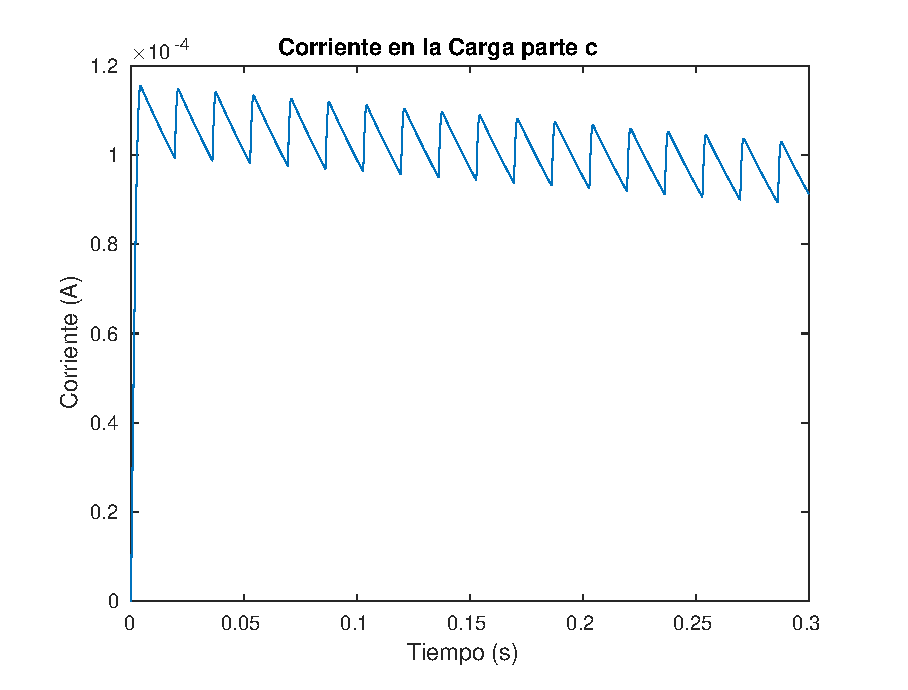
\includegraphics[width=0.8\linewidth]{pictures/Ejercicio2_c_carga.eps}
  \caption{Corriente de carga}
  \label{fig:2_c_carga}
\end{figure}

A partir de la gráfica de la figura \ref{fig:2_c_carga} se puede decir que la corriente en la carga varía al igual que el voltaje de salida, de modo que tampoco parece ser muy significativo, si se piensa en la temperatura a la que tuvo que llegar la temperatura para hacer un poco más apreciable su efecto se puede dar cuenta de que probablemente el circuito estaría derretido pues (1200 K-$926 ^o C$) es una temperatura bastante elevada.


\section{Ejercicio 3}

\subsection{S-Function para el modelo del cohete}
Para la creación de la S-Function del modelo del cohete, en primer lugar se procedió a configurar la
función \texttt{setup} indicando la información sobre la cantidad y tipo de entradas, salidas,
parámetros y estados.

Una vez hecho esto, se establecieron las condiciones iniciales para los estados en la función
\texttt{InitConditions}. De esta manera, se configuró que tanto la altura como la velocidad inicial
del cohete fueran 0 y que la masa inicial fuera la indicada por uno de los parámetros del bloque en
Simulink, tal como se muestra en el siguiente segmento del código.

\begin{lstlisting}[style=Matlab-editor, basicstyle=\mlttfamily]
  function InitConditions(block) %Se inicializan los estados
    % Altura inicial
    block.ContStates.Data(1) = 0;
    % Velocidad inicial
    block.ContStates.Data(2) = 0;
    % Masa inicial
    block.ContStates.Data(3) = block.DialogPrm(7).Data;
\end{lstlisting}

Posteriormente, se programó la función \texttt{Outputs} para calcular las salidas del sistema, las
cuales corresponden a la altura y la velocidad del cohete. De esta forma, se crearon variables
intermedias para almacenar los valores de los estados de altura y velocidad, y también se estableció la
condición de que si se detecta que la altura deja de ser positiva o nula, se fuerce tanto la altura
como la velocidad a 0, tal como se muestra en el siguiente código.

%Salidas
\begin{lstlisting}[style=Matlab-editor, basicstyle=\mlttfamily]
  function Outputs(block) % Se calculan las salidas
    h = block.ContStates.Data(1);
    v = block.ContStates.Data(2);

    % Altura mayor o igual a 0
    if (h < 0)
      block.OutputPort(1).Data = 0;
      block.OutputPort(2).Data = 0;
    else
      block.OutputPort(1).Data = h;
      block.OutputPort(2).Data = v;
    end
\end{lstlisting}

Por otro lado, se configuró la función \texttt{Derivatives}, la cual se encarga de establecer los
valores de las derivadas de los estados del modelo en cada instante de la simulación. De esta
manera, se crearon las variables intermedias para almacenar los estados y los parámetros
del sistema. Luego, se programó la condición de que si la masa del combustible se agota entonces que
la misma se mantenga en un valor de 0, forzando también la tasa de consumo de combustible a 0 en
dicha situación.

Finalmente, se estableció el vector de derivadas, el cual almacena en cada una de sus entradas el
valor correspondiente a la ecuación respectiva del modelo en variables de estado del cohete.

%Derivadas
\begin{lstlisting}[style=Matlab-editor, basicstyle=\mlttfamily]
  function Derivatives(block) % Se calculan las derivadas
    % Estados
    h = block.ContStates.Data(1);
    v = block.ContStates.Data(2);
    mp = block.ContStates.Data(3);

    % Parametros
    ms = block.DialogPrm(1).Data;
    g = block.DialogPrm(2).Data;
    rho = block.DialogPrm(3).Data;
    A = pi*(block.DialogPrm(4).Data)^2;
    ve = block.DialogPrm(5).Data;
    Cd = block.DialogPrm(6).Data;

    % Masa del combustible mayor a 0
    if mp > 0
      up = block.InputPort(1).Data;
    else
      up = 0;
      block.ContStates.Data(3) = 0;
      mp = block.ContStates.Data(3);
    end

    % Derivada h
    block.Derivatives.Data(1) = v;
    % Derivada v
    block.Derivatives.Data(2) = (-(ms+mp)*g + up*ve -(1/2)*rho*v*abs(v)*A*Cd)/(ms+mp);
    % Derivada mp
    block.Derivatives.Data(3) = -up;     
\end{lstlisting}


\subsection{Simulación del movimiento del cohete}
Para el segundo apartado de este ejercicio, se utilizó la S-Function creada dentro de un diagrama de
bloques del programa Simulink, con el cual se simuló la respuesta del modelo del cohete ante una
entrada escalón de 5 segundos que indica la tasa de consumo de combustible del cohete. En la figura
\ref{fig:diag_simulink}, se muestra el diagrama de Simulink utilizado, en el cual se observa que el
bloque de la S-Function efectivamente presenta una entrada y dos salidas, tal como se estableció en
la programación de la función. Los datos de la altura y la velocidad del cohete se capturaron con el
bloque \texttt{Scope}.

\begin{figure}[ht!]
  \centering
  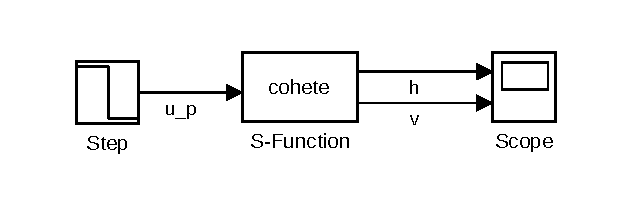
\includegraphics[width=0.5\linewidth]{pictures/Ejercicio3/simulink_cohete.eps}
  \caption{Diagrama de bloques en Simulink}
  \label{fig:diag_simulink}
\end{figure}

En la figura \ref{fig:alt_cohete}, se muestra la gráfica de la altura resultante de la
simulación. De esta forma, la altura empieza incrementado rápidamente, pero luego del instante $t=5$
la concavidad de la curva cambia debido a que la velocidad del cohete empieza a disminuir ya que se
agota el combustible. Posteriormente, la altura llega a un valor máximo para luego disminuir debido
a que la velocidad se vuelve negativa por el efecto de la aceleración de la gravedad. Finalmente, la
altura llega a $h=0$ y se mantiene en ese valor, lo cual indica que el cohete colisionó con el suelo.


\begin{figure}[ht!]
  \centering
  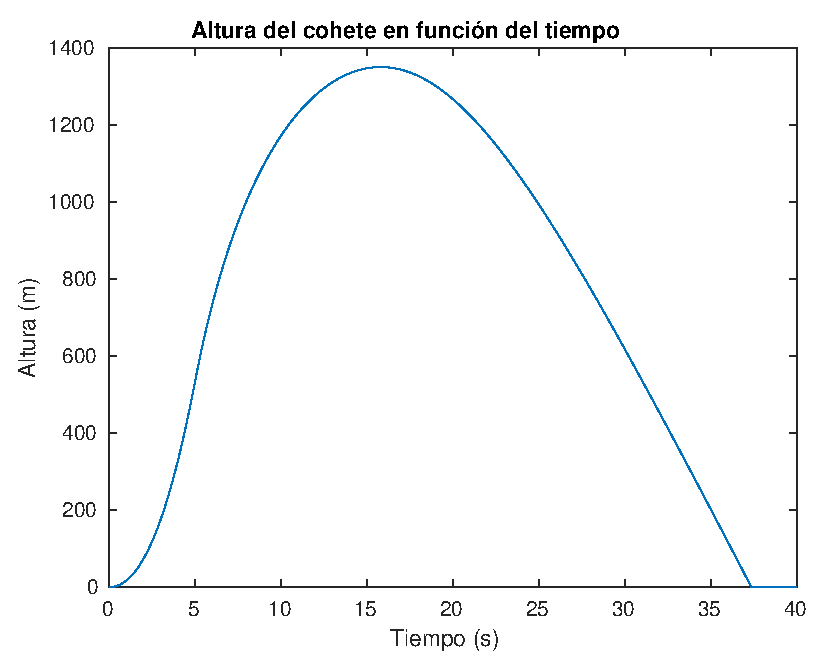
\includegraphics[width=0.5\linewidth]{pictures/Ejercicio3/altura_cohete_vs_tiempo.eps}
  \caption{Gráfica de la altura del cohete con respecto al tiempo}
  \label{fig:alt_cohete}
\end{figure}

En la figura \ref{fig:vel_cohete}, se observa la curva de la velocidad del cohete, además de la
entrada escalón del sistema. Se puede ver como la velocidad llega a un valor máximo que coincide con
el instante en donde se deja de aplicar la entrada del sistema, por lo que el combustible deja de
impulsar el cohete hacia arriba y la aceleración de la gravedad provoca entonces que la velocidad
empiece a disminuir. Posteriormente, la velocidad pasa a ser negativa llegando a un valor casi
constante debido a que la resistencia del aire modelada con el término
$-\frac{1}{2}\rho v(t)|v(t)| A C_D$ en la ecuación de la derivada de la velocidad del MVE provoca
que se llegue a una velocidad terminal. Finalmente, cuando la altura del cohete regresa a $h=0$, se
observa como la condición programada causa que la velocidad cambie súbitamente a $v=0$ debido al
choque con la tierra.

\begin{figure}[ht!]
  \centering
  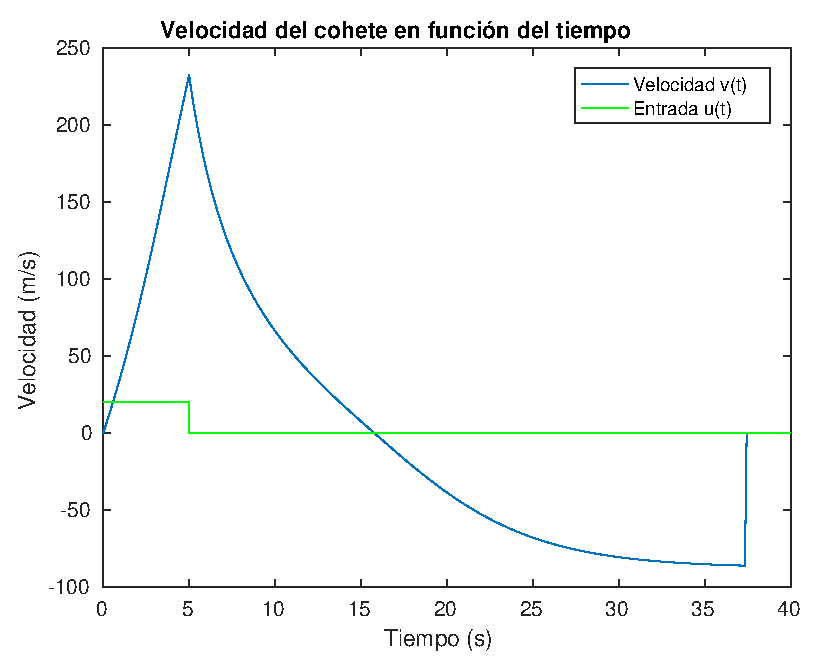
\includegraphics[width=0.5\linewidth]{pictures/Ejercicio3/velocidad_cohete_vs_tiempo.eps}
  \caption{Gráfica de la velocidad del cohete con respecto al tiempo}
  \label{fig:vel_cohete}
\end{figure}







\end{document}
